% Options for packages loaded elsewhere
\PassOptionsToPackage{unicode}{hyperref}
\PassOptionsToPackage{hyphens}{url}
%
\documentclass[
  12pt,
  oneside]{book}
\usepackage{lmodern}
\usepackage{setspace}
\usepackage{amsmath}
\usepackage{ifxetex,ifluatex}
\ifnum 0\ifxetex 1\fi\ifluatex 1\fi=0 % if pdftex
  \usepackage[T1]{fontenc}
  \usepackage[utf8]{inputenc}
  \usepackage{textcomp} % provide euro and other symbols
  \usepackage{amssymb}
\else % if luatex or xetex
  \usepackage{unicode-math}
  \defaultfontfeatures{Scale=MatchLowercase}
  \defaultfontfeatures[\rmfamily]{Ligatures=TeX,Scale=1}
\fi
% Use upquote if available, for straight quotes in verbatim environments
\IfFileExists{upquote.sty}{\usepackage{upquote}}{}
\IfFileExists{microtype.sty}{% use microtype if available
  \usepackage[]{microtype}
  \UseMicrotypeSet[protrusion]{basicmath} % disable protrusion for tt fonts
}{}
\makeatletter
\@ifundefined{KOMAClassName}{% if non-KOMA class
  \IfFileExists{parskip.sty}{%
    \usepackage{parskip}
  }{% else
    \setlength{\parindent}{0pt}
    \setlength{\parskip}{6pt plus 2pt minus 1pt}}
}{% if KOMA class
  \KOMAoptions{parskip=half}}
\makeatother
\usepackage{xcolor}
\IfFileExists{xurl.sty}{\usepackage{xurl}}{} % add URL line breaks if available
\IfFileExists{bookmark.sty}{\usepackage{bookmark}}{\usepackage{hyperref}}
\hypersetup{
  pdftitle={Spatial Pattern Mining of Tech Clusters of Dynamics and Industry Mix Based On Quantitative Methods in England Area, UK},
  hidelinks,
  pdfcreator={LaTeX via pandoc}}
\urlstyle{same} % disable monospaced font for URLs
\usepackage[left=4cm, right=3cm, top=2.5cm, bottom=2.5cm]{geometry}
\usepackage{longtable,booktabs}
% Correct order of tables after \paragraph or \subparagraph
\usepackage{etoolbox}
\makeatletter
\patchcmd\longtable{\par}{\if@noskipsec\mbox{}\fi\par}{}{}
\makeatother
% Allow footnotes in longtable head/foot
\IfFileExists{footnotehyper.sty}{\usepackage{footnotehyper}}{\usepackage{footnote}}
\makesavenoteenv{longtable}
\usepackage{graphicx}
\makeatletter
\def\maxwidth{\ifdim\Gin@nat@width>\linewidth\linewidth\else\Gin@nat@width\fi}
\def\maxheight{\ifdim\Gin@nat@height>\textheight\textheight\else\Gin@nat@height\fi}
\makeatother
% Scale images if necessary, so that they will not overflow the page
% margins by default, and it is still possible to overwrite the defaults
% using explicit options in \includegraphics[width, height, ...]{}
\setkeys{Gin}{width=\maxwidth,height=\maxheight,keepaspectratio}
% Set default figure placement to htbp
\makeatletter
\def\fps@figure{htbp}
\makeatother
\setlength{\emergencystretch}{3em} % prevent overfull lines
\providecommand{\tightlist}{%
  \setlength{\itemsep}{0pt}\setlength{\parskip}{0pt}}
\setcounter{secnumdepth}{5}
\usepackage[none]{hyphenat}
\pagestyle{plain}
\raggedbottom
\usepackage[nottoc,notlot,notlof]{tocbibind}
\usepackage{pdfpages}
\usepackage[width=\textwidth]{caption}

\usepackage{fancyhdr}
\pagestyle{fancy}
\fancyhf{}
\setlength{\headheight}{15pt}%
\fancyhead[RO,RE]{\nouppercase{\leftmark}}
\fancyfoot[CO, CE] {\thepage}
\renewcommand{\headrulewidth}{0pt}
\renewcommand{\footrulewidth}{0pt}
\usepackage{booktabs}
\usepackage{longtable}
\usepackage{array}
\usepackage{multirow}
\usepackage{wrapfig}
\usepackage{float}
\usepackage{colortbl}
\usepackage{pdflscape}
\usepackage{tabu}
\usepackage{threeparttable}
\usepackage{threeparttablex}
\usepackage[normalem]{ulem}
\usepackage{makecell}
\usepackage{xcolor}
\ifluatex
  \usepackage{selnolig}  % disable illegal ligatures
\fi
\usepackage[style=apa,]{biblatex}
\addbibresource{book.bib}
\addbibresource{packages.bib}

\title{Spatial Pattern Mining of Tech Clusters of Dynamics and Industry Mix Based On Quantitative Methods in England Area, UK}
\author{Zeqiang Fang\\
~\\
CASA0012, MSc Spatial Data Science and Visualisation Dissertation\\
~\\
Supervisor: Dr Max Nathan\\
~\\
Repository: \url{https://fang-zeqiang.github.io/CASA0012-Dissertation/}\\
~\\
This dissertation is submitted in part requirement for the\\
MSc in the Centre for Advanced Spatial Analysis,\\
Bartlett Faculty of the Built Environment, UCL\\
~\\
Word count: 8,000}
\date{2021-08-22}

\begin{document}
\maketitle

\setstretch{1.5}
\pagenumbering{roman}

\hypertarget{abstract}{%
\chapter*{Abstract}\label{abstract}}

Some abstract text

word count: 7258

\pagenumbering{roman}

\hypertarget{declaration}{%
\chapter*{Declaration}\label{declaration}}

I, Zeqiang Fang, hereby declare that this dissertation is all my own original work and that all sources have been acknowledged. It is xxx words in length

\hypertarget{acknowledgements}{%
\chapter*{Acknowledgements}\label{acknowledgements}}

I would like to thank blah blah

% Trigger ToC creation in LaTeX
\setcounter{tocdepth}{3}
\tableofcontents
\listoffigures
\listoftables

\hypertarget{abbreviations}{%
\chapter*{Abbreviations}\label{abbreviations}}

\begin{table}
\centering
\begin{tabular}{ll}
\toprule
\textbf{Term} & \textbf{Abbreviation}\\
\midrule
Travel to Work Area & TTWA\\
Herfindahl-Hirschman Index & HHI\\
Local Indicators of Spatial Association & LISA\\
Ordinary Least Squares & OLS\\
\bottomrule
\end{tabular}
\end{table}

\hypertarget{introduction}{%
\chapter{Introduction}\label{introduction}}

\pagenumbering{arabic} 

\hypertarget{background}{%
\section{Background}\label{background}}

\begin{enumerate}
\def\labelenumi{\arabic{enumi}.}
\tightlist
\item
  tech cluster development
\end{enumerate}

\url{https://technation.io/report2021/\#uk-trends}
tech cluster \& ttwa
In fact, between 2007 and 2014, the number of creative enterprises grew faster than the overall company population in more than nine out of ten of the UK's 228 Travel-to-Work-Area geographies (Mateos-Garcia,2016).

There are high clustering effect among the England tech firms

By modeling the evolution of business growth and entry, this research contrasts the dynamics of the process by which regional clusters emerge in the US and UK computer industries. New enterprises are lured to both countries by industrial strength in specific sub-sectors in specific regions. Furthermore, incumbent firms in a cluster that is strong in their particular sub-sector of the industry expand at a quicker rate than the industry average. While there are significant second-order variations between the models estimated for the United States and the United Kingdom, the clustering dynamics appear to be comparable. There is no evidence that clustering effects are weaker in the United Kingdom than in the United States(Baptista and Swann, 1999).

\begin{enumerate}
\def\labelenumi{\arabic{enumi}.}
\setcounter{enumi}{1}
\tightlist
\item
  dynamics cause better performance
\end{enumerate}

dynamics and entry pattern
Many industrial dynamics patterns appear to be shaped by the process by which knowledge is created, gathered, and subsequently destroyed, because it favors the admission of new enterprises, the coexistence of incumbents and new entrants, and, eventually, their selective or combined exit over time (Krafft,2004).

\begin{enumerate}
\def\labelenumi{\arabic{enumi}.}
\setcounter{enumi}{2}
\tightlist
\item
  industry clustering pattern and economics performances
\end{enumerate}

\hypertarget{research-question-and-objectives}{%
\section{Research Question and Objectives}\label{research-question-and-objectives}}

How does tech clusters' dynamics pattern change in UK from 1998 to 2018? / What factors can affect tech clusters' dynamics pattern change in UK?

To what extent will dynamic change affect tech clusters'performance?

Governments all across the world aim to grow their ICT sectors. As a result, researchers and policymakers want a comprehensive image of digital firms, but traditional datasets and typologies lag real-world change. We perform an alternative analysis for all active enterprises in the UK, focused on ICT-producing firms, using innovative ``big data'' resources.
(Nathan and Rosso, 2015)

The approach of spatial autocorrelation analysis is useful for revealing the structure and patterns of economic geographical variables. It can be used to identify not only the country's overall spatial patterns, but also specific micro-locations (Stankov \& Dragićević, 2015).

\hypertarget{report-structure}{%
\section{Report Structure}\label{report-structure}}

\begin{enumerate}
\def\labelenumi{\arabic{enumi}.}
\tightlist
\item
  data clean
\item
  tech cluster recognition
\item
  dynamics index generation
\item
  hypothesis (OLS estimation)
\item
  regression
\item
  residual analysis
\item
  result interpretation
\end{enumerate}

\hypertarget{lit-review}{%
\chapter{Literature Review}\label{lit-review}}

\hypertarget{industry-cluster-tech-cluster}{%
\section{Industry Cluster \& Tech Cluster}\label{industry-cluster-tech-cluster}}

Tech clusters like Silicon Valley play a central role for modern innovation, business competitiveness, and economic performance. This paper reviews what constitutes a tech cluster, how they function internally, and the degree to which policy makers can purposefully foster them. We describe the growing influence of advanced technologies for businesses outside of traditional tech fields, the strains and backlash that tech clusters are experiencing, and emerging research questions for theory and empirical work.

They find ICT employment shares nearly double the usual estimates using their unique `sector-product' approach, however this conclusion is more speculative (ICT production space is around 42 percent larger than SIC-based estimates, with around 70,000 more companies)
(Nathan \& Rosso, 2015)

\hypertarget{cluster-dynamics}{%
\section{Cluster Dynamics}\label{cluster-dynamics}}

Industrial dynamics and clusters: a survey, regional research. This article reviews clusters and their impact on the entry, exit, and growth of firms, as well as the literature supporting the evolutionary dynamics of cluster formation. This extensive review shows strong evidence that clusters promote the entry of manufacturers, but the evidence that clusters can promote the growth and survival of firms is rather weak. From a number of open-ended questions, this research extracts various future research paths that emphasize the importance of manufacturer heterogeneity and the exact mechanism that supports the localized economy (Frenken, Cefis and Stam, 2014).

Relative researchers found that industry clustering not only increased firm entry but also firm exit rates. This implied that clusters could emerge and exist because they provide entry opportunities but they do not necessarily generate Marshallian economies that increase firm survival (Boschma, 2015).

by looking at how clusters influence entry, departure, and growth via localization economics, and by taking a long-term look at cluster emergence and evolution.

Entry is strongly influenced by clustering. Empirical research have consistently found that as cluster size grows, so does the rate of admission. Most potential entrepreneurs simply stay in their region of origin, therefore this empirical correlation does not imply that enterprises locate in a cluster because they gain from co-location.

Localization economies appear to play a role in entrance decisions in these research, but only for technologically trailing businesses who stand to gain the most and have the least to lose from co-location (ALCCER and CHUNG, 2007).

Cluster effect on the whole England area
Enterprise entry does play an important role in shaping the overall dynamics. The new entrants that survive in the cluster will become larger over time, resulting in broader expansion and overall impact (Clementi \& Palazzo, 2016)
\url{https://pages.stern.nyu.edu/~gclement/Papers/Entry_exit.pdf}

\hypertarget{industry-mix}{%
\section{Industry Mix}\label{industry-mix}}

On average, companies in large cities are more productive. There are two main explanations: corporate choice (big cities strengthen competition and only allow the most productive people to survive) and agglomeration economies (big cities promote interaction and increase productivity), which may be strengthened by the natural advantages of localization. In order to distinguish them, we nested a general version of the easy-to-handle company selection model and a standard agglomeration model. Stronger choices in large cities cut the distribution of productivity to the left, while stronger gatherings move to the right and expand the distribution. Using this forecast, French firm-level data, and new quantile methods, we show that firm choices cannot explain differences in spatial productivity. The results are applicable to various departments, city size thresholds, institutional samples and regional definitions.

The Herfindahl--Hirschman Index (HHI) is a commonly used economic concept in competition law, antitrust{[}1{]}, and technology management. It's a measure of a company's size in relation to the industry it's in, as well as an indicator of how competitive it is \hspace{0pt}(Liston-Heyes \& Pilkington, 2004).

\hypertarget{how-location-affect-entry-pattern-in-ukglobal}{%
\section{How location affect entry pattern in UK/Global}\label{how-location-affect-entry-pattern-in-ukglobal}}

\hypertarget{how-time-affect-entry-pattern-in-ukglobal}{%
\section{How time affect entry pattern in UK/Global}\label{how-time-affect-entry-pattern-in-ukglobal}}

\hypertarget{other-factor-can-affect-dynamics-pattern-in-uk}{%
\section{Other factor can affect dynamics pattern in UK}\label{other-factor-can-affect-dynamics-pattern-in-uk}}

Firm density has a beneficial effect on entry rates in the early stages of an industry since each firm has the potential to bring in new entrants. Legitimation has been coined to describe this positive density impact. Higher company density levels, on the other hand, become a barrier to entrance as the industry evolves and grows, owing to fierce market competition (Boschma, 2015).

The empirical evidence reveals that technology and the stage of the industry life cycle impact the relationship between business size and the likelihood of survival.(Agarwal and Audretsch, 2001)
Entry may be less about radical innovation and more about filling strategic niches in established businesses that are nonetheless technologically intensive, neutralizing the impact of entry size on the likelihood of survival.(ibid)

Over time, smaller factories generated proportionately more jobs, implying that job-growth incentives to larger enterprises may have been misdirected. Overall, our findings suggest that the impacts of size and age on manufacturing plant expansion in a developing economy are similar to those in rich economies (negative relationship between plant age and plant growth )(Liu, Tsou and Hammitt, 1999)

\begin{quote}
Firms Growth and Failure
\end{quote}

Moreno's research found that the failure rate and growth rate of companies decline with the growth of scale and age. Regression-to-the-mean is not an important factor in the negative correlation between the size and growth of surviving companies. And he also offers empirical evidence of firm failure rates as well as the mean of the distribution of realized growth rates(Fariñas and Moreno, 2000).
\url{https://sci-hub.se/10.1023/A:1007834210622}
Fariñas, J. and Moreno, L., 2000. Review of Industrial Organization, 17(3), pp.249-265.

\hypertarget{methodology}{%
\chapter{Methodology}\label{methodology}}

\hypertarget{research-framework}{%
\section{Research Framework}\label{research-framework}}

The study area is 149 travel to work areas in England, UK (Figure \ref{fig:fig-study-area}). The areas in blue colour is the main research area. In this study, a data set containing all companies in UK will be cleaned and attribute selected, and technology companies will be identified and screened according to the classification and definition of technology companies on the official website of the British government. Before the quantitative study, this study is based on time and The spatial dimension counts the number of technology companies, and calculates the dynamic indicators of enterprise clusters and industrial combination indicators in a specific year and a specific region. Then this study conducts multiple regressions, univariate variables Moran index testing to conduct spatial quantitative research, and finally combines Qualitative spatial pattern trend research on the spatial changes of indicators in three different time periods(1998, 2008 \& 2018).

\begin{figure}
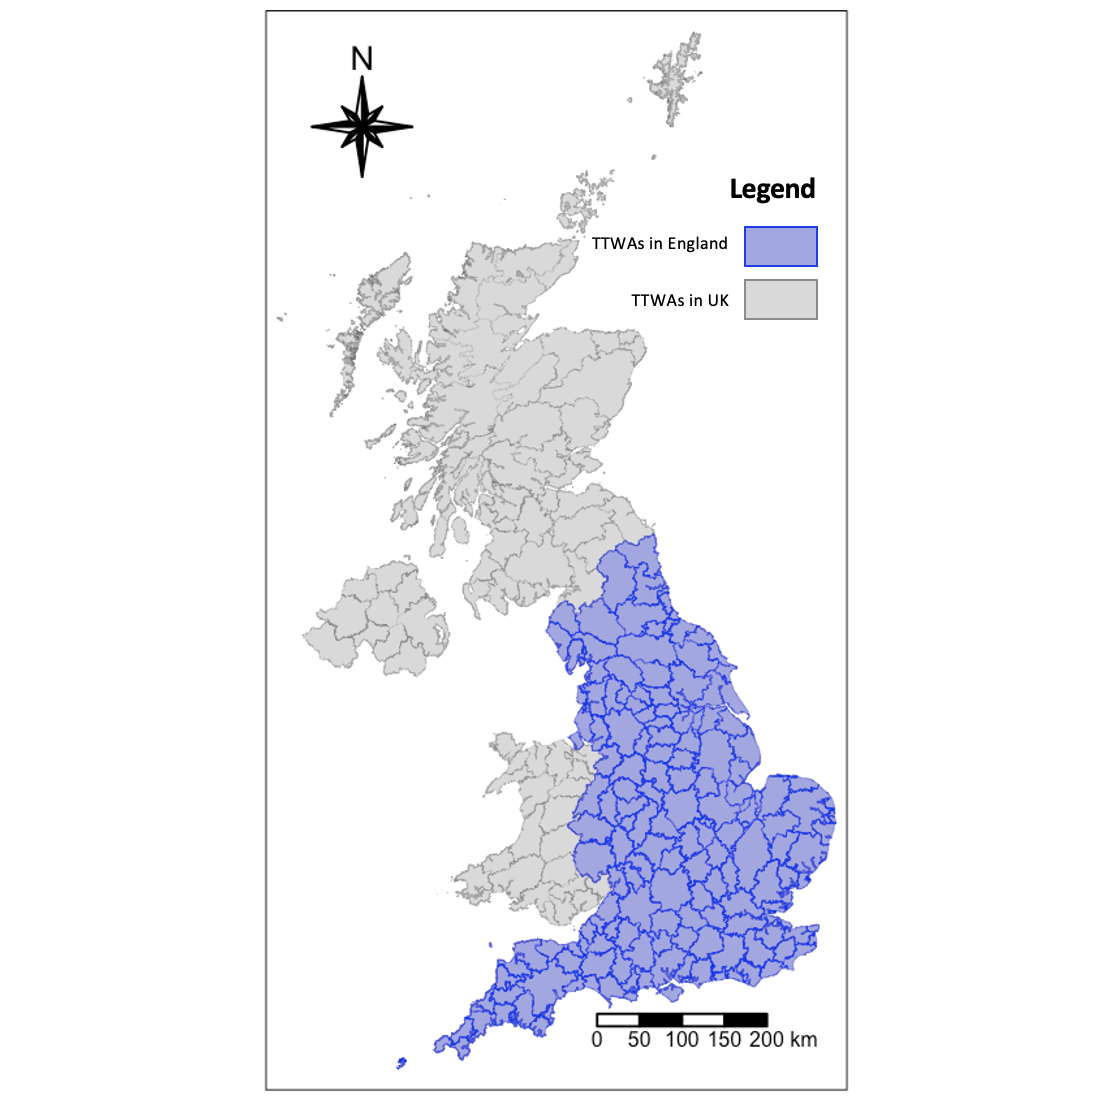
\includegraphics[width=1\linewidth]{/Users/fangzeqiang/Github/CASA0012-Dissertation/bookdown/general_images/study_area} \caption{The Map of Travel to Work Areas (TTWAs) within UK}\label{fig:fig-study-area}
\end{figure}

\hypertarget{data-source-and-processing}{%
\section{Data Source and Processing}\label{data-source-and-processing}}

This raw dataset is collected from the core company data from Open Corporates master company database (Open Corporates, 2018). And the size of dataset accounts for 15 GB which is handled with \texttt{read\_stata} and \texttt{get\_chunk} function to read large data file in chunks, then increasing the reading speed. The ``primary uk sic 2007'' identification field is the basis of industry finding and the ``birth year'' is the key to measure dynamics variables . All rows whose these two values are empty are removed(17\% incorperate date is missing and sic code is complete).

\hypertarget{identifying-tech-clusters}{%
\section{Identifying Tech Clusters}\label{identifying-tech-clusters}}

For the identification of science and technology companies, this study introduces the main 2007 sic code table to judge the science and technology industry, referring to the classification method of the Science and Technology Classification data set on the ons.gov.uk website. In order to better identify science and technology companies for the UK. The economic contribution is officially based on the 2007 British Standard Economic Activity Classification, different data sources were combined to classify and label science and technology companies (Office for National Statistics, 2015).The 5-digital sic code can identify the economic activity classification of the technology industry in the finest granularity. The statistics bureau provided a comparison table of sic codes for the classification of science and technology industries, which can help this research to better identify technology companies from the big data of UK companies (\ref{tab:tab-sic-part}).

\begin{longtable}[t]{>{\raggedright\arraybackslash}p{3cm}>{\raggedright\arraybackslash}p{3cm}>{\raggedright\arraybackslash}p{3cm}}
\caption{\label{tab:tab-sic-part}Science and Technology Classification Sample (Part)}\\
\toprule
\textbf{5-digit SIC07 code} & \textbf{Science and Technology category} & \textbf{Science and Technology topic}\\
\midrule
26110 & Digital Technologies & Computer \& Electronic manufacturing\\
58210 & Digital Technologies & Digital \& Computer Services\\
62090 & Digital Technologies & Digital \& Computer Services\\
63110 & Digital Technologies & Digital \& Computer Services\\
27510 & Other scientific/technological manufacture & Electrical Machinery manufacturing\\
\addlinespace
… & … & …\\
86230 & Life Sciences \& Healthcare & Healthcare services\\
\bottomrule
\end{longtable}

This research refers to the science and technology classification table provided by the government. The technology indicator is used to position the technology industry of all industries, and a total of 168 sic codes for the technology industry in 2007 were obtained, accounting for about 16\% of all industry categories in the UK, including 5 industry categories such as Digital Technologies, Life Sciences \& Healthcare, Publishing \& Broadcasting , Other scientific/technological manufacture and Other scientific/technological services, details of the classification form will be attached in the attachment. There are almost 20\% firms in the raw data belonging to tech firms according to the method of category as mentioned above.

\hypertarget{data-scale}{%
\section{Data Scale}\label{data-scale}}

\hypertarget{time-range-selection}{%
\subsection{Time Range Selection}\label{time-range-selection}}

The reason why this research choose tech firms which incorporate from 1998 to 2018 is because the number of technology companies established in the UK in the past 20 years is significantly higher than before 1998, as shown in below figure.

\begin{figure}
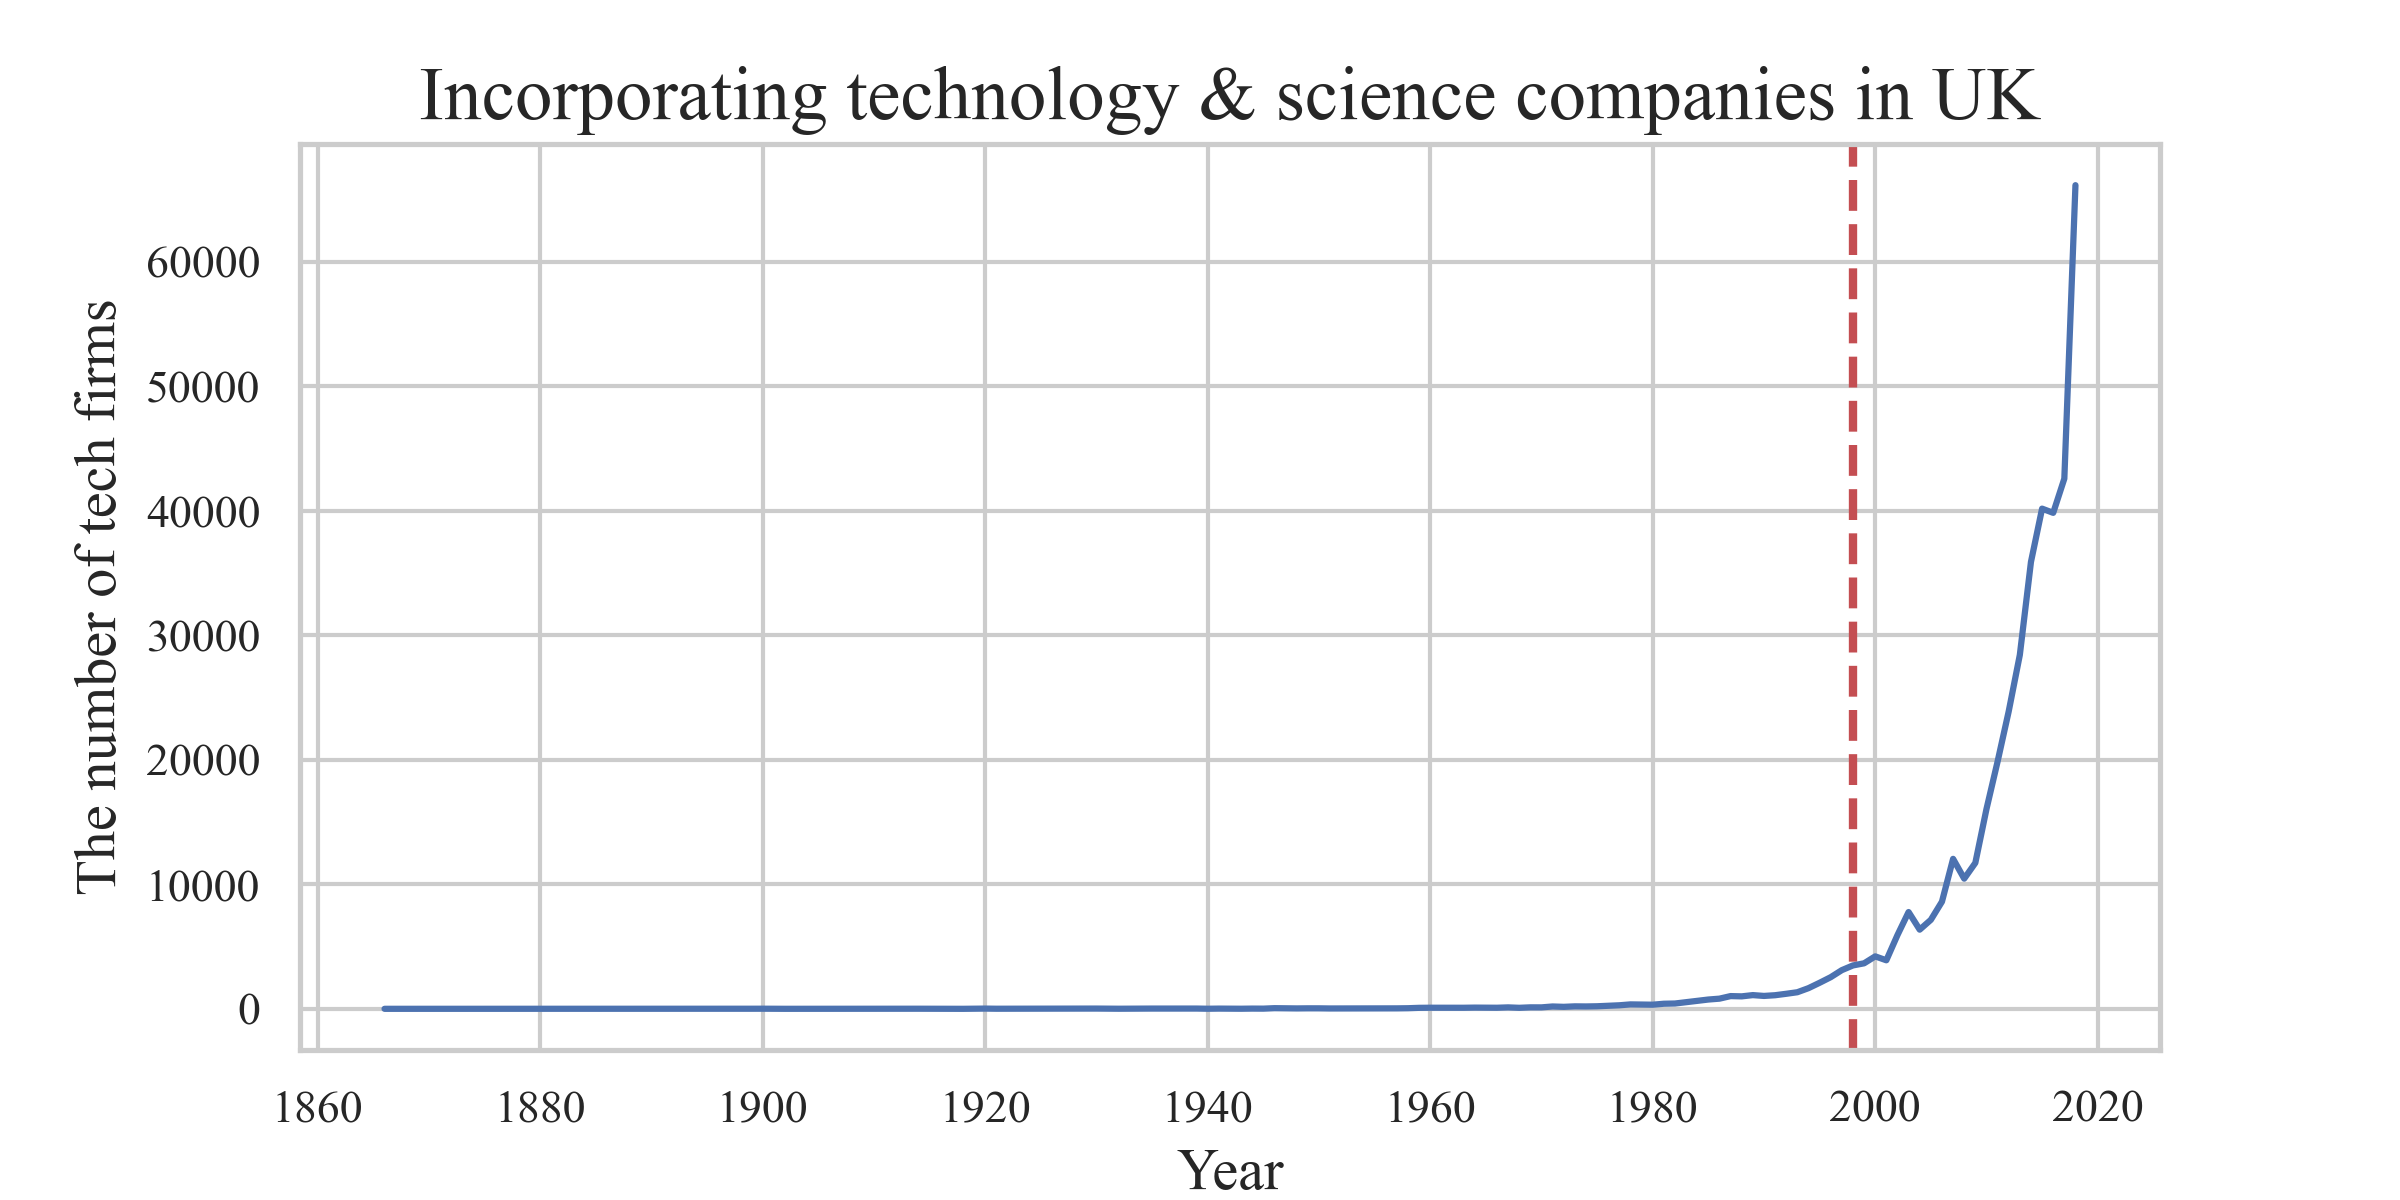
\includegraphics[width=1\linewidth]{/Users/fangzeqiang/Github/CASA0012-Dissertation/bookdown/general_images/figure1} \caption{Incorporating technology and science companies in UK}\label{fig:fig-1}
\end{figure}

\hypertarget{tech-cluster-identifying}{%
\subsection{Tech Cluster Identifying}\label{tech-cluster-identifying}}

Travel to Work Locations is official statistics that capture local labour markets, i.e., areas where the majority (approximately 70\%) of the people who live there work. These measures are based on responses to the 2011 and are used to define the TTWAs algorithmically. There are currently 228 TTWAs in the UK. When it is recognised that the activity of interest may be scattered across administrative boundaries such as local authority districts or NUTS areas, TTWAs are widely utilised in industrial clustering investigations (Prothero, 2021).

Relevant studies have shown that commuting across towns has become more common in England and Wales. People are not limited to living and working in the same administrative area. In addition, studies have found that low-skilled workers tend to rely on the public to work locally. Strong skill-oriented jobs are more dependent on cars, and they are also the main force for cross-city commuting. The technology industry has a greater demand for those strong skill-oriented workers which suggest that travel to work area(TTWA) is used as a cluster of technology companies compared to traditional administrative Region would be a good choice (Titheridge \& Hall,2006)

The University of Cambridge had funded some researchers to undertake the Wisbech 2020 Vision project to analyse the current problem, mining the potential future space for employment growth with alternative macro-economic scenario to help drive a high value-added growth plan in the local area (Burgess \& et al., 2014)

This geographical division can better reflect the relationship between population, company and work. In terms of geographic research, related researchers have combined the Business Structure Database (BSD) from the Office for National Statistics (ONS) and industry classification methods to use the ONS geographic area of TTWA to survey the commuting patterns and labour market of the population in 2011. Most scholars state that this might be an effective measure for the research of industrial clusters at the sub-regional level (Mateos-Garcia,2016).

\hypertarget{quatitative-analysis-and-methods}{%
\section{Quatitative Analysis and Methods}\label{quatitative-analysis-and-methods}}

\hypertarget{dynamics-measuring-index}{%
\subsection{Dynamics Measuring Index}\label{dynamics-measuring-index}}

Firm entry is the result of the interaction between the
characteristics of an actor, on the one hand, and the surrounding environment, on the other hand (Frenken, Cefis and Stam, 2014).

To measure the degree of dynamic change of a cluster, it is necessary to calculate the entry rate of the technology cluster. Brandt used the enterprise's entry rate and exit rate to measure the dynamics attributes of a company (2005). This research refers to the researcher's calculation method. The number of enterprises entering and quitting a sector as a percentage of the total number of firms in the same sector in a given year is used to compute entry rate in this tech cluster dynamics research(ibid). The calculation method is as follows.

\[ 
Entry\ Rate_{i,t} = \frac{Incorporating\ Firms_{i,t}}{Total\  Firms_{i}} 
\]

Where \(i\) means location(travel to work area), \(t\) means year

\hypertarget{industry-mix-measuring-index}{%
\subsection{Industry Mix Measuring Index}\label{industry-mix-measuring-index}}

It is necessary to calculate the Herfindahl-Hirschman Index or location quotient of the technology cluster to measure the degree of industrial concentration in a cluster area. However, only the former method is used because the employment data corresponding to the corresponding region year is missing; Here is a reference to the quantitative method of industrial concentration of Chao Lu's research team (2017). HHI is calculated by squaring the market share of each competing company and then adding the results, where the market share is given in the form of scores or points (ibid). Increases in the Herfindahl index generally indicate a decrease in competition and an increase of market power, whereas decreases indicate the opposite (Hall \& et al., 2009), as the calculation method shown below.

\[
HHI_{\ i,t} = \sum_{j=1}^N (\frac{Tech\ Firms_{j,i,t}}{Total\ Tech\ Firms_{i,t}})^2 
\]
Where:
\(HHI_{i,t}\) means Herfindahl-Hirschman ~Index in location \(i\) and year \(t\)

\(N\) is the overall number of individual tech firm contained.

\(k\) represents the \(k\)th industry in location \(i\) and year \(t\).

\(Tech Firms_j\) is the number of j-th individual tech firm

\(Total Tech Firms\) represents the number of total tech firms in a specific location and year.

\hypertarget{regression}{%
\subsection{Regression}\label{regression}}

In order to quantify the impact of industry concentration and company density in the cluster on the cluster dynamic variable (entry rate), the Herfindahl-Hirschman Index and company density corresponding to the year and location(i.e.~ttwa) in the data are used as independent variables (Table \ref{tab:tab-reg-idp-var}). And the variable of the numeric data type of entry rate is regarded as the dependent variable

\begin{table}

\caption{\label{tab:tab-reg-idp-var}Independent Variables Selection for Regression}
\centering
\begin{tabular}[t]{lll}
\toprule
\textbf{Independent Variables} & \textbf{Type} & \textbf{Description}\\
\midrule
Density & numeric & The density of tech firms\\
Herfindahl-Hirschman Index & numeric & The index measuring the industry mix\\
Year & category & Years from 1998 to 2018\\
Location & category & Top ten clusters of companies in England\\
\bottomrule
\end{tabular}
\end{table}

Dynamics variable(entry rate) is measured empirically by the ratio of the number of new firms at the end of a period to the total number of firms at the beginning of the period(Hause \& Du Rietz, 1984), unless otherwise stated. The equation regression model is given:

\[
\ y\ =\ b_0 + b_1 \ x_1 + b_2 \ x_2 + \sum_{i=3}^{4} \ b_i \ x_i + \epsilon_{i,j}
\]
Where

\(y\) means entry rate in the year and location
\(x_1\) means the year, a dummy variable
\(x_2\) means location, i.e.~travel to work area(TTWA)
\(x_3\) means the density of tech firms in a specific year and location
\(x_4\) means Herfindahl-Hirschman Index in in a specific year and location
\(\epsilon_{i,j}\) is a random error.

\hypertarget{global-autocorrelation-morans-i}{%
\subsection{Global Autocorrelation (Moran's I)}\label{global-autocorrelation-morans-i}}

One of the most popular and often used measures of spatial autocorrelation is Moran's Index. Based on the locations and values of the feature, the Global Moran's I tool analyzes the pattern of a data set spatially and decides if it is scattered, clustered, or random. The program calculates the Moran's I Index value, as well as the z-score and p-value, to statistically validate the Index. It is computed using the formula below (Kumari \& et al., 2019).

\[
Moran's \ I = \frac{n}{S_0} \frac{\sum_{x=1}^n \sum_{y=1}^n w_{x,y} z_x z_y}{\sum_{x=1}^n z_x^2}
\]
\[
S_0 = \sum_{x=1}^n \sum_{y=1}^n w_{x,y}
\]

Where \(z_x\) stands for deviation of an attribute from its mean \((x_i – X̅)\) for feature \(X\), \(w_{x,y}\) is the spatial weight among feature \(X\) and \(Y\), \(n\) is the total number of features and So is the summation of all spatial weights

The statistic's \(z_j\) score is given below

\[ 
z_x = \frac{I - E[I]}{\sqrt{V[I]}}
\]
where

\[
E[I] = \frac{-1}{(n-1)}
\]

\[
V[I] = E[I^2]-E[I]^2
\]

The Moran's Index(I) has a range of values from -1 to 1. Index value 1 indicates that the observed pattern is spatially clustered. On the other hand value -1 indicates scattering or dispersion. Moran's I assign a value of near or equal to zero to the lack of auto correlation. The z-score and p-value of the Index are only used to form final judgments regarding the observed pattern. Besides, local indicators of spatial association will be applied to measure the high-high and low-low clusters(Anselin, 2010). According to research method of Kumari's team(2019), the Moran's I of three time period will be calculated to analysis the dynamics change in spatial and temporal aspects.

\hypertarget{hot-spot-analysis-getis-ord-gi}{%
\subsection{Hot-Spot Analysis (Getis-Ord Gi*)}\label{hot-spot-analysis-getis-ord-gi}}

Only positive spatial autocorrelation is taken into account by the local Getis statistics, which allows for discrimination between clusters of similar values that are high or low relative to the mean. The Getis--Ord local statistics are calculated as follows by Getis \& Ord (2010):

\[
G^*_j = \frac{\sum_{j=1}^nw_{i,j}x_j - \bar{X}\sum_{j=1}^{n}w_{i,j}}{S\sqrt{\frac{[n\sum_{j=1}^{n}w^2_{i,j} - (\sum_{j=1}^{n}w_{i,j})^2)]}{n-1}}}
\]

where \(x_j\) is the attribute value for feature \(j, w_{i,j}\) is the spatial weight between feature \(i\) and \(j\), \(n\) is equal to the total number of features and:

\[ 
\bar{x} = \frac{\sum_{j=1}^{n}x_j}{n}
\]

\[
S = \sqrt{\frac{\sum_{j=1}^{n}x^2_j}{n} -(\bar{x})^2}
\]

The Gi* statistic returned for each feature in the dataset is a z-score (Getis \& Ord, 2010). For statistically significant positive z-scores, the larger the z-score is, the more intense the clustering of high values (hot spot). For statistically significant negative z-scores, the smaller the z-score is, the more intense the clustering of low values (cold spot).

\hypertarget{limitations}{%
\section{Limitations}\label{limitations}}

In term of missing value in the original dataset, there are almost 99.8\% missing value in dissolution date. This means that most companies do not have a dissolution date, which might not mean that some companies survive, nor can it accurately reflect the company's exit numbers in a specific year and region. Moreover, the company's incorporation date data (including firms birth year) is also missing about 17.26\%. These two difficulties make the data after cleaning process may have the risk of insufficient accuracy in representing the dynamics of the industry. The model prediction after fitted to this dataset might not reach the same situation as the real world level.

England travel to work areas might not be a data-driven method to identify the clusters. This spatial boundary data is not an up-to-date dataset because it is lastly updated in 2015. Changes in commuting have pushed TTWA boundaries further since their inception in the 1980s. With the passage of time, the boundaries of TTWA will be further changed in the future due to changes in commuting methods(Ozkul,2014) which might make this research slightly inappropriate in the future application.

The value of this statistical data(Herfindahl-Hirschman Index) for identifying monopoly development, on the other hand, is directly dependent on the precise definition of a market (Kwoka, 1977). For instances, geographical considerations might influence market share. This dilemma can arise when there are nearly equal market share of tech businesses in a given sector, but they each operate exclusively in distinct regions of the travel to work area, resulting in each firm having a monopoly inside the specific marketplace in which it conducts business, which might make it more difficult to measure the industry mix in a specific location and year. Furthermore, one IT firm may control as much as 70\% of the market for a certain area of the digital industry (i.e.~the sale of one specific equipment). As a result, that company would have a near-total monopoly on the manufacturing and sale of that commodity.

\hypertarget{ethical-statement}{%
\section{Ethical Statement}\label{ethical-statement}}

The data for this project comes from OpenCorporates, a firm which aggregates company-level data from around the world(\url{https://opencorporates.com/}). In this case, OpenCorporates have taken data from the UK Companies House register (\url{https://www.gov.uk/government/organisations/companies-house}). As detailed by Nathan and Rosso (2015), all limited companies in the UK need to registers with Companies House when they are set up, and provide annual returns and financial statements. These include details of directors and company secretary, registered office address, shares and shareholders, as well as company type and principal business activity. Thus, all the data used here is already in the public domain.

The research objectives are tech firms in the UK for this project and the individual data will not be collected and measured in this project. For issues of deanonymisation or privacy, traceable information such as the real companies name and ID will not be utilised in the research. The raw data will be cleaned and filtered by several key variables include industries instead of the company's name or other sensitive information before doing the research. Through data cleaning, pre-processing, desensitisation or other processing methods, the risks of damage to company interests (such as social reputation, economic benefits and etc.) will be mitigated to an as low as possible level in the research process.

Besides, this project will not cause discrimination of industries or job categories. The final analysis results, such as the different industry concentration in each region, will not deepen some people's stereotypes and prejudices about the region (This content will be fully discussed in the project discussion section). It is necessary to point out and declare the objectivity of the analysis and the non-absoluteness of the results in the disclaimer. Consider the feelings of people and governments in different parts of the UK, this research will prevent the influence of personal preferences and subjective emotions.

The leakage of companies' name and information will be protected. For example, in the reflection of the results section of academic research, the name and related information of the companies that moved may be revealed. Although this information may be open to the public you need to know that this information may be used by people with other ulterior motives. This project will desensitise the company name and information at the stage of chart presentation, such as using A, B, and C to replace them to achieve this purpose.

\hypertarget{results}{%
\chapter{Results}\label{results}}

\hypertarget{spatial-and-temporal-distribution}{%
\section{Spatial and Temporal Distribution}\label{spatial-and-temporal-distribution}}

In terms of three variables' change of overall England level,it can be found that the average firms' entry rate and density in England increase significantly(Figure \ref{fig:fig-all-var-trend}). There was a growth in firms entry rate from 0.01(1998) to 0.14(2018) and the statistics of density climb from 0.02 to 0.43 during these decades (Table \ref{tab:tab-all-var-trend}). However, the Herfindahl-Hirschman index decreased by less than 0.1 in 2018 which is 1/3 times than that in 1998. Overall, it can be seen that the dynamics increased but the industry concentration reduced.

\begin{figure}
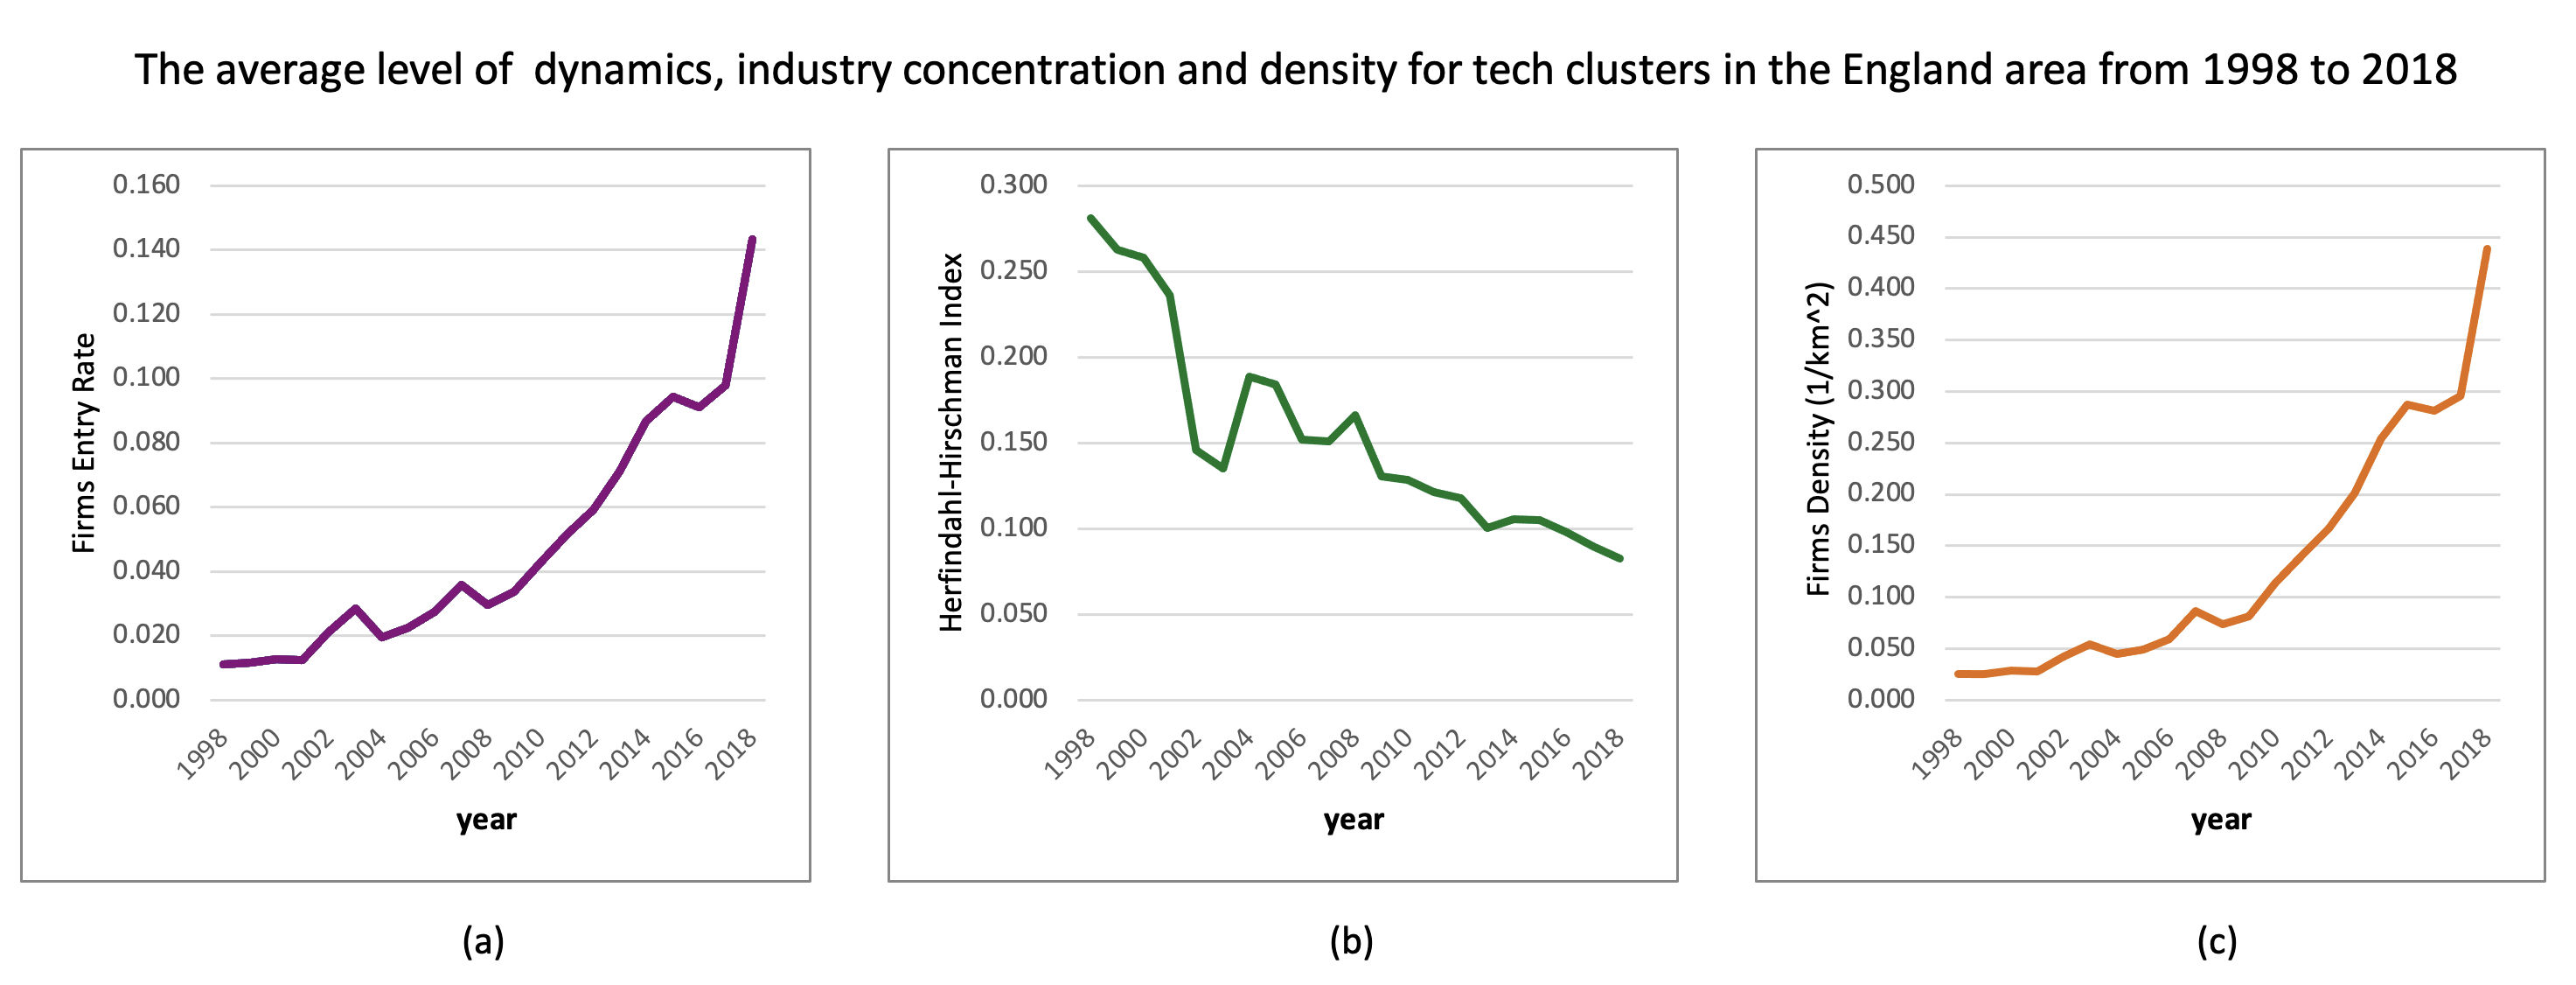
\includegraphics[width=1\linewidth]{/Users/fangzeqiang/Github/CASA0012-Dissertation/bookdown/general_images/all_enR_hh_den_change} \caption{The average level change of three variables in two decades}\label{fig:fig-all-var-trend}
\end{figure}

How to reference (Figure \ref{fig:fig-all-var-trend})

\begin{table}

\caption{\label{tab:tab-all-var-trend}The average level change of three variables in two decades}
\centering
\begin{tabular}[t]{rrrr}
\toprule
\textbf{Year} & \textbf{Entry Rate} & \textbf{Herfindahl-Hirschman Index} & \textbf{Density (1/km\textasciicircum{}2)}\\
\midrule
1998 & 0.0111338 & 0.2811410 & 0.0251467\\
1999 & 0.0116754 & 0.2625985 & 0.0255016\\
2000 & 0.0127544 & 0.2580325 & 0.0288208\\
2001 & 0.0124221 & 0.2361455 & 0.0279131\\
2002 & 0.0212760 & 0.1460459 & 0.0420549\\
\addlinespace
2003 & 0.0285419 & 0.1350075 & 0.0540107\\
2004 & 0.0195123 & 0.1886668 & 0.0449568\\
2005 & 0.0225973 & 0.1841296 & 0.0492084\\
2006 & 0.0274033 & 0.1521901 & 0.0592952\\
2007 & 0.0358175 & 0.1507693 & 0.0862518\\
\addlinespace
2008 & 0.0295100 & 0.1662619 & 0.0737782\\
2009 & 0.0336153 & 0.1305273 & 0.0817783\\
2010 & 0.0425260 & 0.1285513 & 0.1134154\\
2011 & 0.0516425 & 0.1212957 & 0.1404650\\
2012 & 0.0593572 & 0.1179875 & 0.1664194\\
\addlinespace
2013 & 0.0712224 & 0.1006216 & 0.2015662\\
2014 & 0.0867586 & 0.1056914 & 0.2538923\\
2015 & 0.0943852 & 0.1048371 & 0.2869250\\
2016 & 0.0912387 & 0.0980931 & 0.2812983\\
2017 & 0.0979282 & 0.0894585 & 0.2954844\\
\addlinespace
2018 & 0.1432780 & 0.0827082 & 0.4387067\\
\bottomrule
\end{tabular}
\end{table}

How to reference (Table \ref{tab:tab-all-var-trend})

\hypertarget{tech-cluster-dynamics}{%
\subsection{Tech Cluster Dynamics}\label{tech-cluster-dynamics}}

From 1998 to 2018, the entry rate of each Travel to work area (TTWA) in England will change drastically every decades. For example, in 1998 the darker colored areas were mostly around the Greater London area and the entire southern part of England(Figure \ref{fig:fig-enR-1998-2018-v1}). The overall entry rate in 2008 was higher than that in 1998 and showed a trend of new companies entering the north of England. In this year, some travel to work areas on the edge of England have more prominent entry rates, such as Malton, Minehead and Bridport. However, the overall entry rate in 2018 was about twice as high as the average in 2008. Moreover, ttwa with high entry rate is mostly concentrated in the north and the surrounding areas of Greater London. The overall trend can be witnessed as given by Table \ref{tab:tab-all-var-trend} that there is an increasing trend in the overall level of entry rate from 1998 (average about 1.06\% ) to 2018
(average about 14.33\%)

Finally, from the perspective of changes in temporal and spatial distribution, the increase in the entry rate of the travel to work area in the northern part of England is much larger than that in the southern part. The areas with high entry rates before 2008 were mostly scattered in other areas except for the Greater London area. However, close to after 2018, London and its surrounding areas, the central Manchester-Birmingham area and the southwest, such as Exeter, have a rising entry rate. In contrast, in 2008, the urban agglomerations north of Leeds had higher firm entry rates in tech industry(Figure \ref{fig:fig-enR-1998-2018-v1}).

\begin{figure}
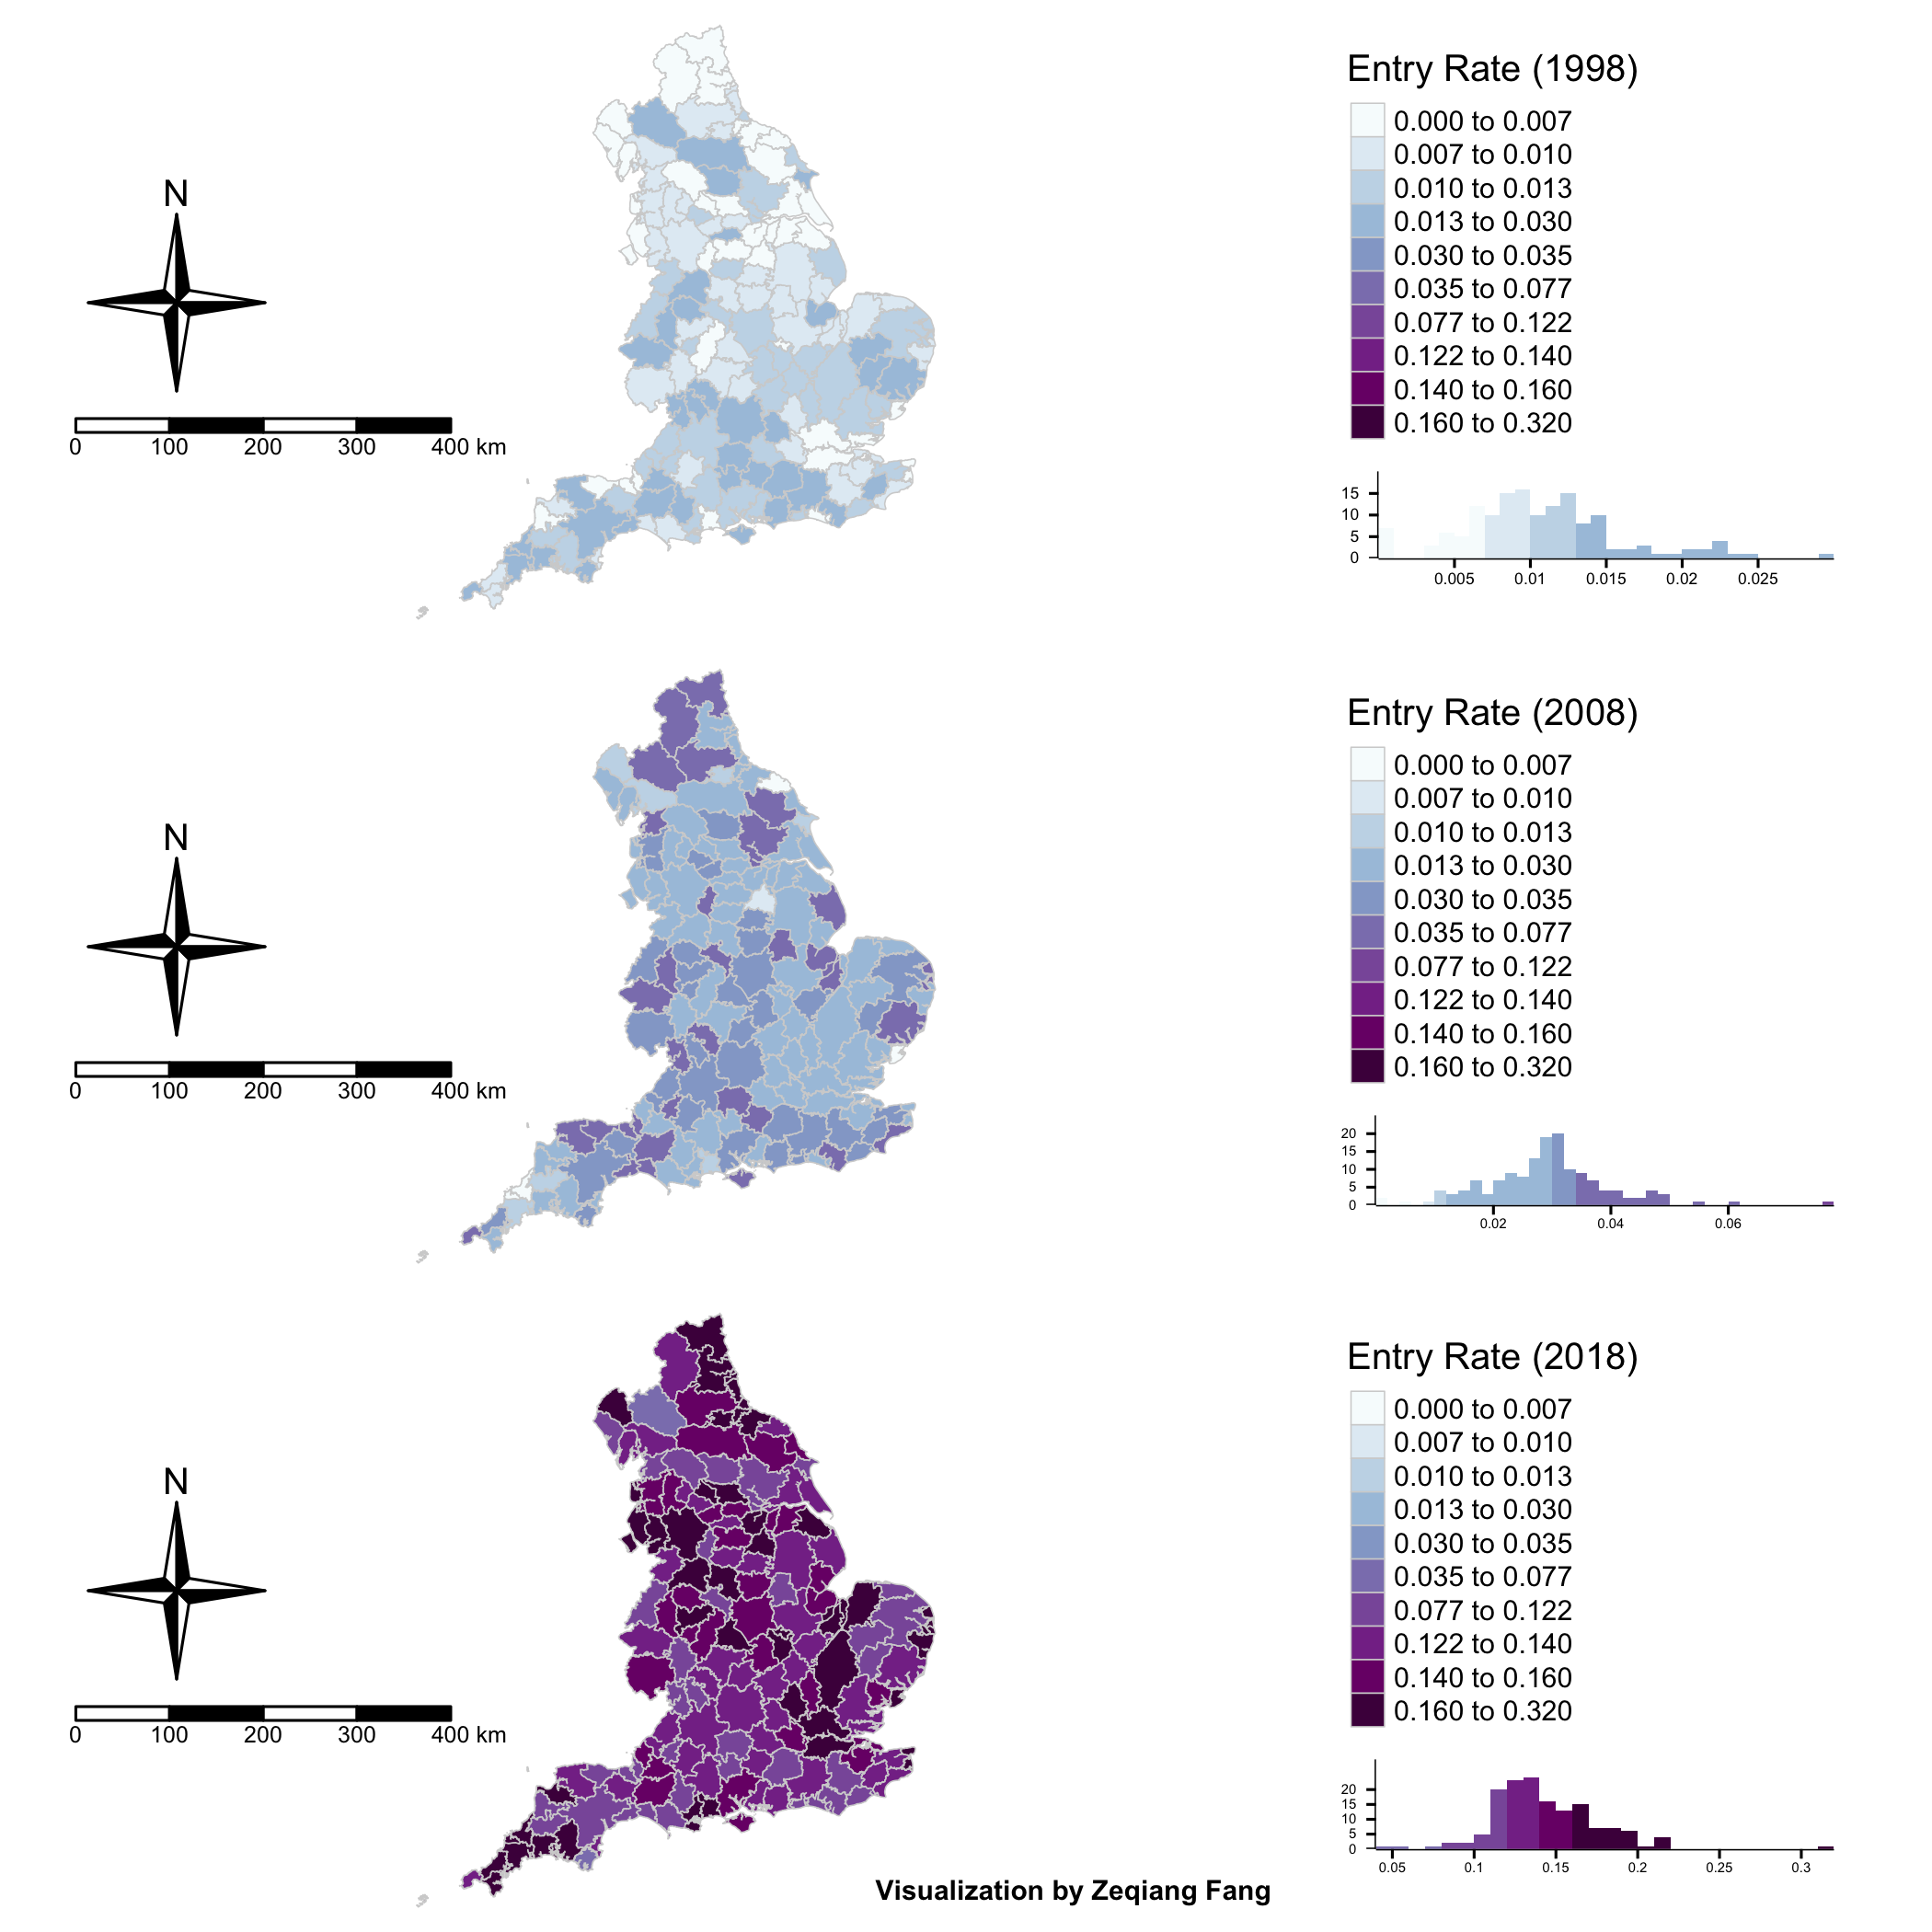
\includegraphics[width=1\linewidth]{/Users/fangzeqiang/Github/CASA0012-Dissertation/bookdown/general_images/enR_1998_2018_v1} \caption{The Distribution of the Firms Entry Rate of the England Travel to Work Areas(TTWAs) from 1998 to 2018}\label{fig:fig-enR-1998-2018-v1}
\end{figure}

\hypertarget{tech-industry-mix}{%
\subsection{Tech Industry Mix}\label{tech-industry-mix}}

In terms of herfindahl-Hirschman index of tech industry in travel to work area of England. As given figure below, it can be seen that the Herfindahl-Hirschman index has a downward trend year by year (Figure \ref{fig:fig-hh-1998-2018}). In the methodology module, this index is mentioned as a measure of industrial concentration. A decrease in the value represents an increase in industrial competition and a decrease in market power. The decline of the index means that the types of SIC codes corresponding to companies in a particular region have increased in a year or the number of companies corresponding to a large share of SIC codes has decreased. In other words, the types of technology industries corresponding to the unit area have increased, or the number of advantageous industries has decreased; you can see The concentration of technology industries out of England declined year by year from 1998 to 2018 (Table \ref{tab:tab-all-var-trend}). In the same way, the diversity of the technology industry is also increasing, and the richness of the industry may also be related to the increase in the entry rate of enterprises.

From the perspective of temporal and spatial distribution, the technology industry was concentrated in northern England, northern and southwestern England before 2008. With the passage of time, even if the concentration of industries in some small areas scattered on the border of England is still high, the Herfindahl-Hirschman index in these places has gradually decreased to a level comparable to that of the Greater London area(Figure \ref{fig:fig-hh-1998-2018}).

\begin{figure}
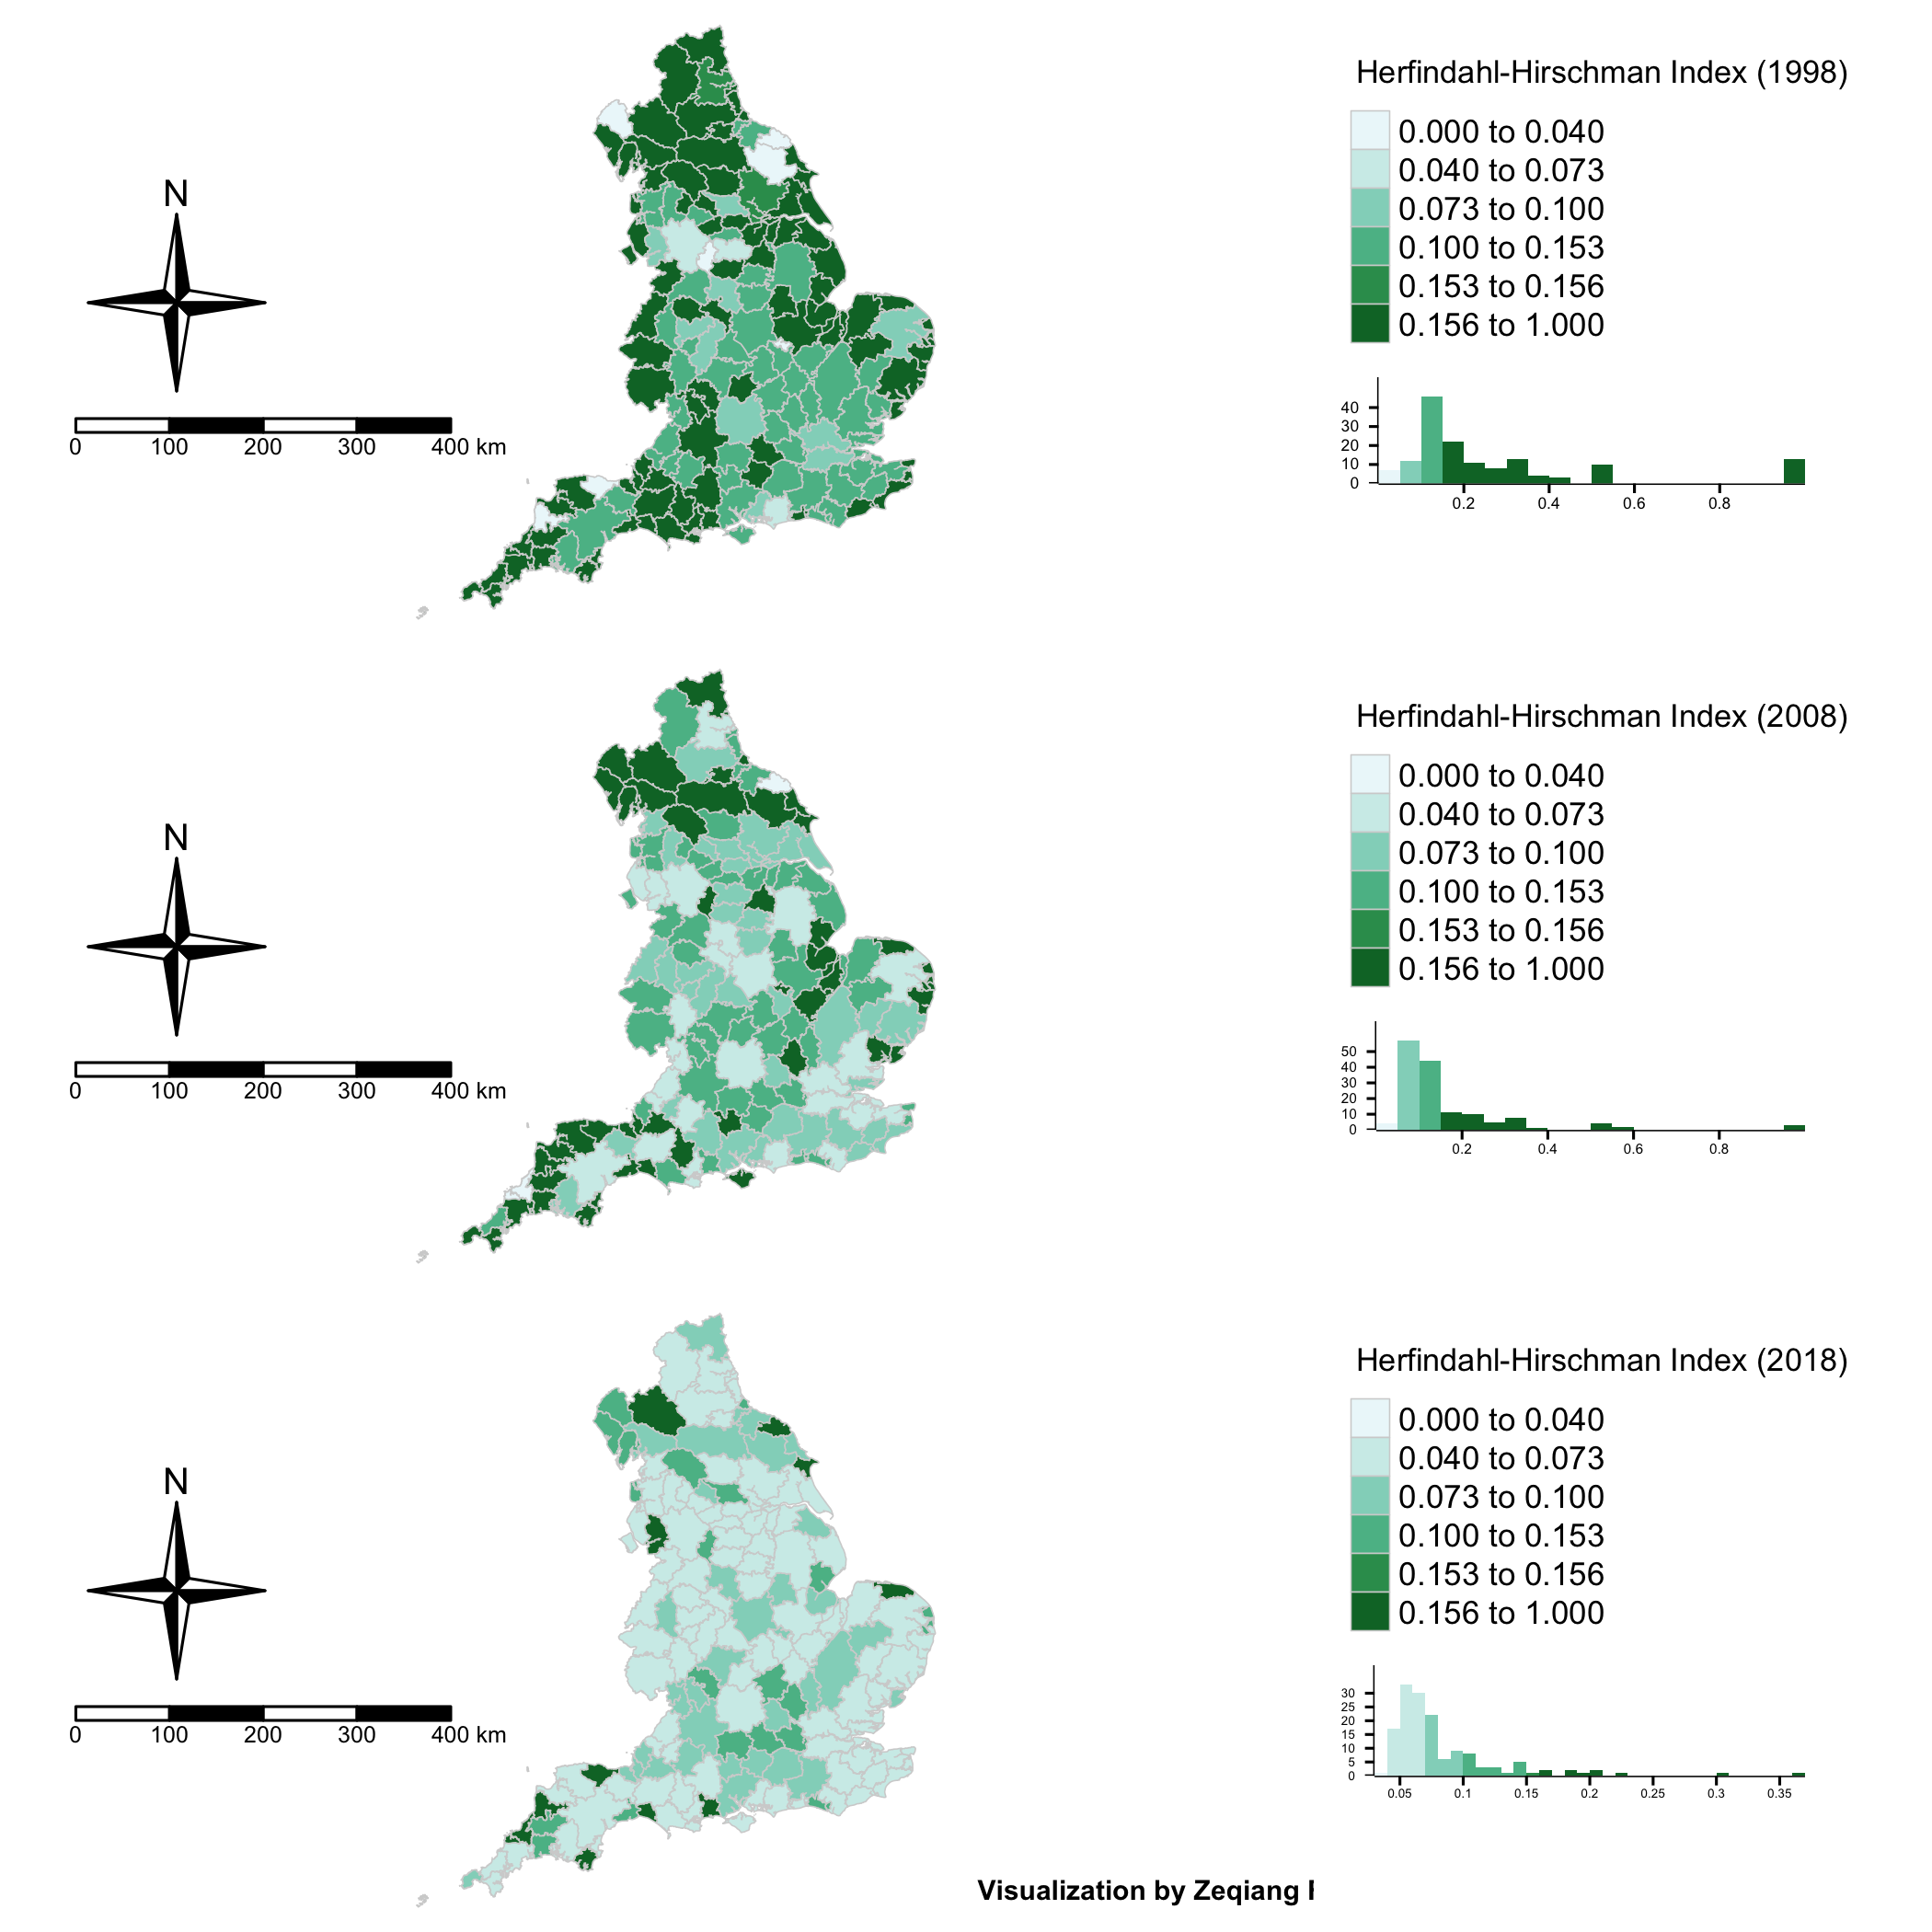
\includegraphics[width=1\linewidth]{/Users/fangzeqiang/Github/CASA0012-Dissertation/bookdown/general_images/hh_1998_2018} \caption{The Distribution of the Herfindahl-Hirschman Index of the England Travel to Work Areas(TTWAs) from 1998 to 2018}\label{fig:fig-hh-1998-2018}
\end{figure}

\hypertarget{regression-analysis}{%
\section{Regression Analysis}\label{regression-analysis}}

For 149 tech clusters(travel to work areas), the regression results can indicate the relationship among cluster dynamics, industry mix and firms density in different years(1998-2018) and locations (149 tech clusters). Among these three models, the model with outliers excluded and logarithmic processing of the dependent variable performed better. It can be seen that the Herfindahl-Hirschman index has a negative correlation with the tech cluster dynamic variable (entry rate) but the density has a positive effect.

Taking Model {[}3{]} as an example, every time this indicator decreases by one unit, the entry rate might increase by about \(e^{1.37}\) unit times higher than the original one. The high confidence of this coefficient can explain 99\% of all observation data. On the contrary, for the density of these tech clusters in Model {[}3{]}, every time the density increases by one unit, the corresponding dependent variable entry rate will be about \(e^{0.5}\) unit times more than the original one (Table \ref{tab:tab-regression-entry-rate}). Although the HHI and Density values of the three models are not the same, the positive and negative effect of the relationship are similar. For example, for the industrial concentration variable HHI, all three models show a negative correlation (Table \ref{tab:tab-regression-entry-rate}). And when HHI and Density change the same unit, the former seems to have a greater impact on the entry rate (it may increase the dependent variable entry rate by more than \(e\) times in both model 1 and model 2)

\begin{table}

\caption{\label{tab:tab-regression-entry-rate}Regression Results of Firms Entry Rate and Tech Clusters' Characters}
\centering
\begin{tabular}[t]{llll}
\toprule
\textbf{Model} & \textbf{{}[1]} & \textbf{{}[2]} & \textbf{{}[3]}\\
\midrule
Method & OLS & OLS & OLS\\
Sample & all areas & all areas & exclude 2018 London\\
Dep. Variable & Entry Rate & Log(Entry Rate) & Log(Entry Rate)\\
\midrule
HHI & -0.0281*** & -1.332*** & -1.3693***\\
 & {}[0.002] & {}[0.045] & {}[0.044]\\
\addlinespace
Density & 0.0168*** & 0.3904*** & 0.504***\\
 & {}[0.001] & {}[0.019] & {}[0.022]\\
Constant & 0.0207* & -4.1138* & -4.0948*\\
 & {}[0.003] & {}[0.068] & {}[0.066]\\
\midrule
Observations & 3089 & 3089 & 3088\\
\addlinespace
R-squared & 0.89 & 0.89 & 0.90\\
\bottomrule
\multicolumn{4}{l}{\textsuperscript{a} All regressions include dummy variables for 149 travel to work}\\
\multicolumn{4}{l}{areas(ttwa) in England and 20 years from 1998 to 2018. Figures in}\\
\multicolumn{4}{l}{brackets are standard errors. ***, **, and * represent statistical}\\
\multicolumn{4}{l}{significance at 1\%, 5\%, and 10\%, respectively.}\\
\multicolumn{4}{l}{\textsuperscript{b} HHI defined by Herfindahl-Hirschman index can indicate the industry}\\
\multicolumn{4}{l}{concentration}\\
\multicolumn{4}{l}{\textsuperscript{c} Source: tech firm data in England travel to work areas from 1998 to}\\
\multicolumn{4}{l}{2008 (n = 3089)}\\
\end{tabular}
\end{table}

As mentioned in the methodology section(Brandt, 2005), Table \ref{tab:tab-regression-control-var} can illustrates the unconditional relation between entry rate and tech cluster characters. These two independent variables are controlled to be added in the regression model which can help to observe to what extent they can have an influence on the dynamics element(entry rate).

When the year and regional conditions in the model remain unchanged, the model {[}1{]} only adds Herfindahl-Hirschman index to consider the regression analysis, and it can be found that the coefficient is about -1.2 and the confidence level is greater than 95\%. Similarly, the model {[}2{]} only considers adding firm density into the fitting, the coefficient of this independent variable is about 0.38 and the statistical significance is also less than 5\%. However, when other conditions are the same, adding two variables into the model at the same time {[}3{]}, the absolute value of each coefficient increases, and the confidence level increases, and the overall goodness of fit is also improved (Table @ref(tab :tab-regression-control-var)).

In terms of Herfindahl-Hirschman index, the entry rate might decrease when this indicator increase(Table \ref{tab:tab-regression-control-var}).
Consistent with model{[}2{]}, the entry rate increase with density (Table \ref{tab:tab-regression-control-var}). The HHI decrease and density increase, leading to lower entry rates.

\begin{table}

\caption{\label{tab:tab-regression-control-var}Regression Results of Firms Entry Rate and Tech Clusters' Characters (variables Controlled)}
\centering
\begin{tabular}[t]{llll}
\toprule
\textbf{Model} & \textbf{{}[1]} & \textbf{{}[2]} & \textbf{{}[3]}\\
\midrule
Method & OLS & OLS & OLS\\
Sample & exclude 2018 London & exclude 2018 London & exclude 2018 London\\
Dep. Variable & Log(Entry Rate) & Log(Entry Rate) & Log(Entry Rate)\\
\midrule
HHI & -1.1844** &  & -1.3693***\\
 & {}[0.047] &  & {}[0.043]\\
\addlinespace
Density &  & 0.3779** & 0.504***\\
 &  & {}[0.025] & {}[0.022]\\
Constant & -4.1884* & -4.5143* & -4.0948*\\
 & {}[0.072] & {}[0.075] & {}[0.066]\\
\midrule
Observations & 3088 & 3088 & 3088\\
\addlinespace
R-squared & 0.884 & 0.869 & 0.901\\
\bottomrule
\multicolumn{4}{l}{\textsuperscript{a} All regressions include dummy variables for 149 travel to work areas(ttwa) in}\\
\multicolumn{4}{l}{England and 20 years from 1998 to 2018. Figures in brackets are standard}\\
\multicolumn{4}{l}{errors. ***, **, and * represent statistical significance at 1\%, 5\%, and}\\
\multicolumn{4}{l}{10\%, respectively.}\\
\multicolumn{4}{l}{\textsuperscript{b} HHI defined by Herfindahl-Hirschman index can indicate the industry}\\
\multicolumn{4}{l}{concentration}\\
\multicolumn{4}{l}{\textsuperscript{c} Source: tech firm data in England travel to work areas from 1998 to 2008 (n =}\\
\multicolumn{4}{l}{3089)}\\
\end{tabular}
\end{table}

\hypertarget{spatial-autocorrelation}{%
\section{Spatial Autocorrelation}\label{spatial-autocorrelation}}

Through the global Moran's Index test of entry rate variable, it can be found that as time increases, the spatial cluster effect of entry rate attribute in England is getting weaker and weaker, from about 0.12 (1998) to 0.05 (2018).

The confidence of global Moran's I in 1998 is as high as 95\%. But the statistical significance of 2008 is lower than 10\%, which indicates weak interpretability of these two years(Table \ref{tab:tab-morans-i-enR}).

\begin{table}

\caption{\label{tab:tab-morans-i-enR}Global Moran's Index of Firms Entry Rate in Three Time Periods}
\centering
\begin{tabular}[t]{rrlr}
\toprule
\textbf{Year} & \textbf{Moran’s Index} & \textbf{p value} & \textbf{z-score}\\
\midrule
1998 & 0.118 & 0.00 & 2.438\\
2008 & 0.062 & 0.08 & 1.348\\
2018 & 0.056 & 0.10 & 1.238\\
\bottomrule
\end{tabular}
\end{table}

Contrary to the entry rate variable, the density attribute value of England has always maintained a relatively obvious spatial aggregation phenomenon, although the global Moran's Index of the density variable has been decreasing year by year. This variable has higher confidence in global Moran's I statistics in the three-year statistics, thus its interpretability is higher than that for mentioned entry rate (Table \ref{tab:tab-morans-i-den}).

\begin{table}

\caption{\label{tab:tab-morans-i-den}Global Moran's Index of Firms Density in Three Time Periods}
\centering
\begin{tabular}[t]{rrlr}
\toprule
\textbf{Year} & \textbf{Moran’s Index} & \textbf{p value} & \textbf{z-score}\\
\midrule
1998 & 0.436 & 0.00 & 10.078\\
2008 & 0.325 & 0.00 & 7.545\\
2018 & 0.189 & 0.00 & 4.982\\
\bottomrule
\end{tabular}
\end{table}

\hypertarget{lisa-analysis-of-firms-dynamics}{%
\subsection{LISA Analysis of Firms Dynamics}\label{lisa-analysis-of-firms-dynamics}}

Local Indicators of Spatial Association(LISA)
According to the Table \ref{tab:tab-z-p-corr}, the z-score with its significance can be found.

\begin{table}

\caption{\label{tab:tab-z-p-corr}Correspondence of Z-score and P-value}
\centering
\begin{tabular}[t]{llr}
\toprule
\textbf{Z-score} & \textbf{p-value} & \textbf{confidence}\\
\midrule
less than -1.65 or more than 1.65 & less than 0.10 & 0.90\\
less than -1.96 or more than 1.96 & less than 0.05 & 0.95\\
less than -2.58 or more than 2.58 & less than 0.01 & 0.99\\
\bottomrule
\end{tabular}
\end{table}

The visualisation result of the local Moran's index's Z-score of Entry rate is as similarly indicated by the global Moran coefficient (Figure \ref{fig:fig-enR-1998-2018-v1}). With the growth of the year, the overall agglomeration effect of England has decreased. But, in this process, the agglomeration effect in the northern region was higher than that in other regions. However, the travel to work areas in the southwest corner changed significantly from the early cluster effect in 1998 to the corresponding outliers such as Low-High, High-Low areas in 2018 (Figure \ref{fig:fig-lisa-entry-rate} ). In addition, from Figure \ref{fig:fig-hh-1998-2018}, the higher industrial concentration in the north also makes the phenomenon of dynamics agglomeration more obvious than that in other places in England area

To be more specific, High-High clusters in 1998 are mainly concentrated in travel to work areas in northern areas such as Newcastle, southern areas such as Andover-Newbury, and the southwest of Exeter. The entry rate values around these places may be higher than the British average. The Low-Low clusters of entry rates are clustered in the northern North Yorkshire area. The surrounding areas of these places usually have relatively close entry rates and low entry rate values;

With the passage of time, the High-High cluster has shifted (the north like Whitehaven and the southwest corner like Launceston areas with higher entry rates gradually formed). By 2018, High-High cluster only appeared in travel to work areas around Liverpool, and new low tech firms entry rate areas were formed in Workington and Penrith\&Appleby (Figure \ref{fig:fig-lisa-entry-rate})

Central regions of England such as London, Birmingham and other regions have not had obvious spatial clustering effects in the visualisation results. This may be due to the low statistical confidence of the local Moran's index among regions. Or it might be because the data in this study is aggregated before calculated. The related data may be missing after the HHI and entry rate are utilised, which might not perfectly represent the company information in some parts of England.

\begin{figure}
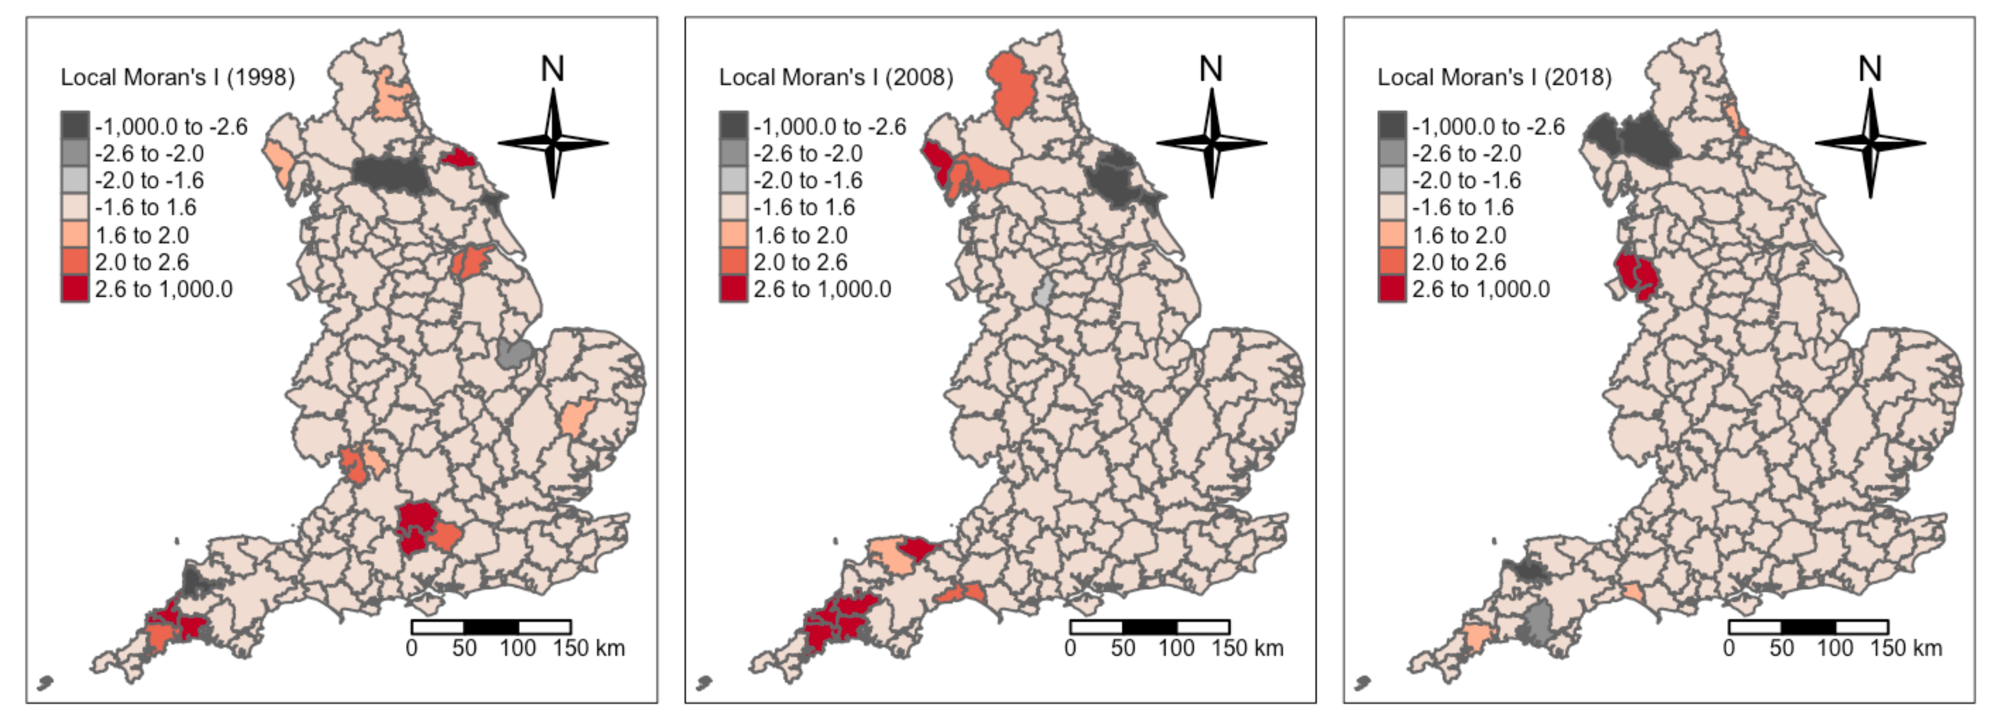
\includegraphics[width=1\linewidth]{/Users/fangzeqiang/Github/CASA0012-Dissertation/bookdown/general_images/Lisa_enR_v1} \caption{Local Moran's I Spatial Analysis for Entry Rate in England for Three Time Periods}\label{fig:fig-lisa-entry-rate}
\end{figure}

\hypertarget{hot-spot-analysis-of-firms-dynamics}{%
\subsection{Hot-Spot Analysis of Firms Dynamics}\label{hot-spot-analysis-of-firms-dynamics}}

This research identified and mapped local clusters (hot and cold spots) by the level of entry rate for these three period.

On the whole, there is a distinct north-south difference in the distribution of cold and hot spots in the early stage(1998). With the development of England tech clusters, this difference is slowly dissipating and a reversal is formed eventually(Figure \ref{fig:fig-Gi-entry-rate}). More specifically, in 1998, there were some hot spots concentrated in the Swindon-Bristol-Reading urban belt in the south-central area and the southwest urban agglomeration of Exeter. Whilst, in the north, there were scattered cold spots represented by the Whitehaven area.

By 2008, most of the hot spots disappeared, and the places that were hot spots gradually became cold spots, such as the southwestern region. In 2018, some hot spots appeared in the northwestern region along with England. The original two hot spots in the southwest have experienced two-time nodes in 2008 and 2018, and they finally turned into cold spot clusters(Figure \ref{fig:fig-Gi-entry-rate}).

From: \url{https://sci-hub.se/10.1556/032.65.2015.3.1}

Discussion: 从时空趋势的角度上看,北方逐渐成为entry rate的热点,有越来越多的科技公司加入北方并且这一现象具有空间自相关性;而西南部地区如何进行政策鼓励和调整来使得他们的科技产业重新焕发生机,税收?

\begin{figure}
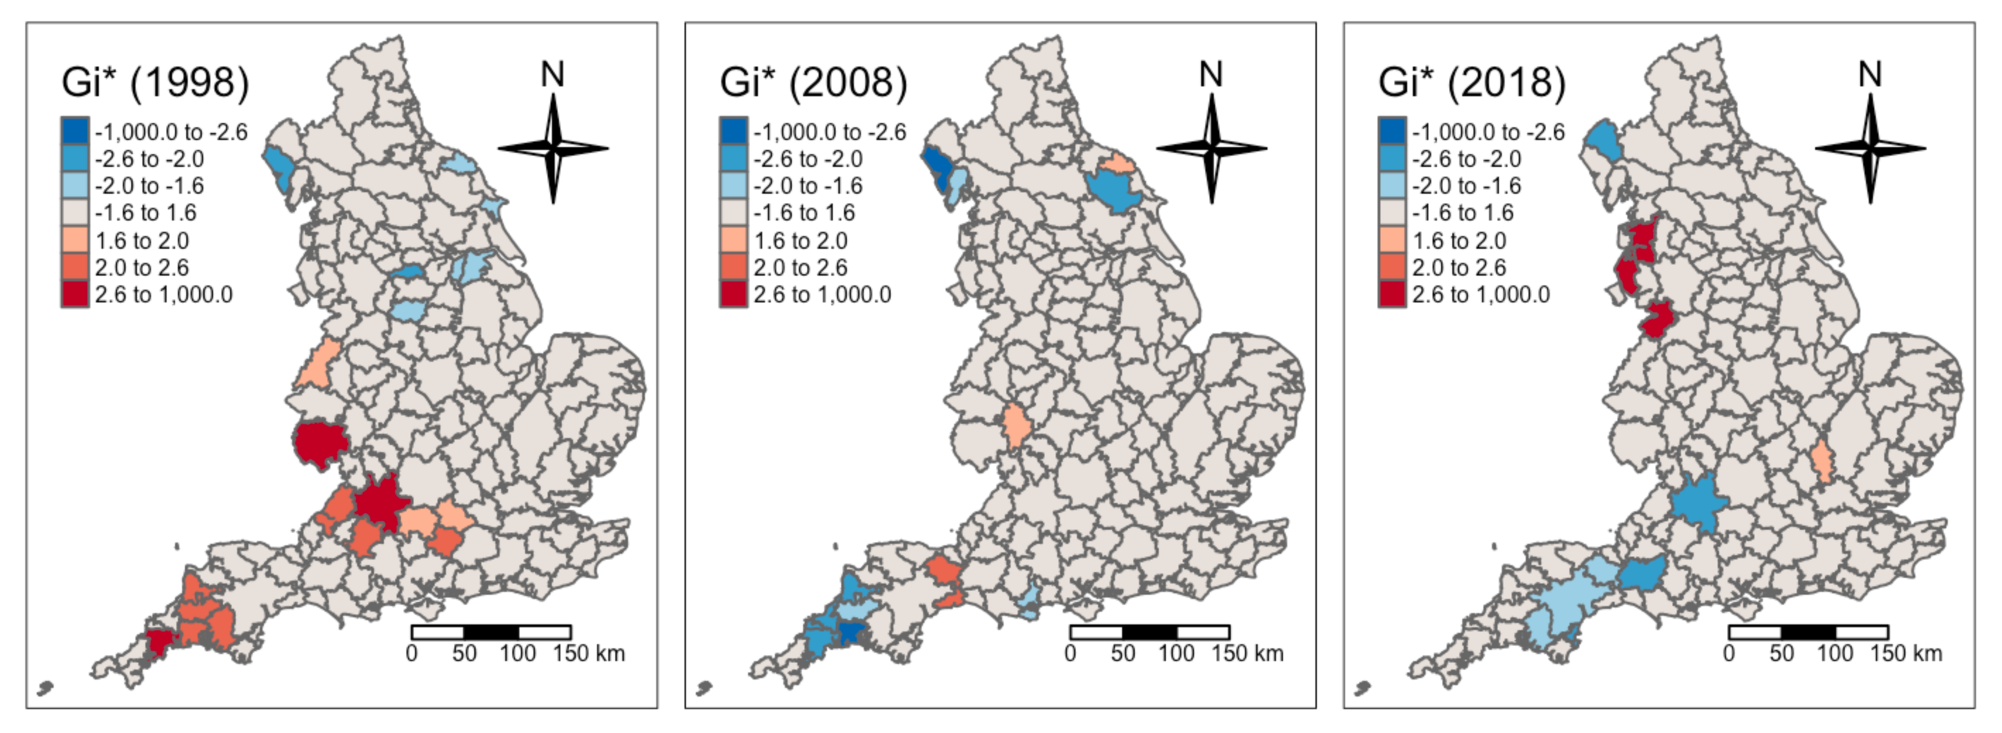
\includegraphics[width=1\linewidth]{/Users/fangzeqiang/Github/CASA0012-Dissertation/bookdown/general_images/G_enR_v1} \caption{Local Gi* Score Statistics for Entry Rate in England for Three Time Periods}\label{fig:fig-Gi-entry-rate}
\end{figure}

\hypertarget{disc}{%
\chapter{Discussion}\label{disc}}

Short introduction to the chapter, reviewing the previous chapter and detailing what this one aims to achieve and build upon.

To be done

\hypertarget{research-significance}{%
\section{Research significance}\label{research-significance}}

\hypertarget{global-development-goals}{%
\subsection{Global development goals}\label{global-development-goals}}

\hypertarget{local-policy}{%
\subsection{Local policy}\label{local-policy}}

\hypertarget{academic-research}{%
\subsection{Academic research}\label{academic-research}}

\hypertarget{limitations-1}{%
\section{Limitations}\label{limitations-1}}

To be done

\hypertarget{transferability}{%
\section{Transferability}\label{transferability}}

To be done

TTWA可以作为\ldots{}

\hypertarget{conclusion}{%
\chapter{Conclusion}\label{conclusion}}

case (Clementi \& Palazzo,2016)
This paper provides a framework to study the dynamics of the cross--section of firms and its implications for aggregate dynamics. When calibrated to match a set of moments of the investment process, our model delivers implications for firm dynamics and for the cyclicality of entry and exit that are consistent with the evidence.

The survival rate increases with size. The growth rate of employment is decreasing with size and age, both unconditionally and conditionally. The size distribution of firms is skewed to the right. When tracking the size distribution over the life a cohort, the skewness declines with age. The entry rate is positively correlated with current and lagged output growth. The exit rate is negatively correlated with output growth and positively associated with future growth.

Carefully modeling firm--level dynamics turns out to be key. The pro--cyclicality of entry and the positive association between age and firm growth deliver amplification and propagation of aggregate shocks in a plain-vanilla competitive framework.

A positive shock to aggregate productivity leads to an increase in entry. Consistent with the empirical evidence, entrants are smaller than incumbents. The skewness of the distribution of firms over idiosyncratic productivity increases. As the exogenous component of aggregate productivity declines towards its unconditional mean, the new entrants that survive grow in productivity and size. That is, the distribution of idiosyncratic productivity improves. As a result, the response of output is stronger and more persistent than in an environment that abstracts from entry and exit.

Our numerical experiments reveal that on average, entry and exit account for about one fifth of the above--trend growth experienced by our economy over the 10 years following a 1.5 standard deviation innovation to aggregate productivity. As an alternative metric of the impact of entry and exit on aggregate dynamics, we assessed the effect on persistence. For a version of our model without entry or exit to generate a data--conforming persistence of output, the first--order auto correlation of aggregate productivity shocks must be 0.775. In the benchmark scenario with entry and exit, it needs only be 0.685.

Last, but not least, we show that according to our model there is a clear causal link between the exceptionally large drop in establishments during the great recession and the painfully low speed of the recovery from it. Whatever its exact nature, the adverse event that initiated the recession had a particularly strong effect on the 2008 and 2009 cohorts, severely reducing the ranks of small but high--conditional--growth plants and thereby suppressing the growth in aggregate labor demand for years to come.

In spite of the wealth of detail and descriptive realism achieved by the model, our framework could be extended in a variety of dimensions. In particular, we would like to gauge the quantitative effect of our mechanism when imbedded in a genuine general equilibrium framework. Relaxing our assumption that firms of different cohorts share the same technology is also of interest. Assuming, as it appears to be the case in reality, that entrants are more likely to adopt more recent vintages of capital, is likely to further enhance the amplification and propagation mechanism uncovered here.
end (Clementi \& Palazzo,2016)

\hypertarget{references}{%
\chapter*{References}\label{references}}
\addcontentsline{toc}{chapter}{References}

a b c d e f g h i j k l m n o p q r s t u v w x y z

Alcacer J. and Chung W., 2007 Location strategies and knowledge spillovers, Management Science 53, 760--776.

Anselin, L., 2010. Local Indicators of Spatial Association-LISA. Geographical Analysis, 27(2), pp.93-115.

Agarwal, R. and Audretsch, D., 2001. Does Entry Size Matter? The Impact of the Life Cycle and Technology on Firm Survival. Journal of Industrial Economics, 49(1), pp.21-43.

Brandt, N., 2005. Business dynamics and policies. OECD Economic Studies, 2004(1), pp.9-36.

Burgess, G., Monk, S., Morrison, N. and Udagawa, C., 2014. Economic Analysis of the Wisbech Travel to Work Area: Main Report: March 2014.

Baptista, R. and Swann, G., 1999. A comparison of clustering dynamics in the US and UK computer industries. Journal of Evolutionary Economics, 9(3), pp.373-399.

Boschma, R., 2015. Do spinoff dynamics or agglomeration externalities drive industry clustering? A reappraisal of Steven Klepper's work. Industrial and Corporate Change, 24(4), pp.859-873.

Combes, P.-P., Duranton, G., Gobillon, L., Puga, D. and Roux, S. (2012),The Productivity Advantages of Large Cities: Distinguishing AgglomerationFrom Firm Selection. Econometrica, 80: 2543-2594.https://doi.org/10.3982/ECTA84427

Clementi, G.L. and Palazzo, B., 2016. Entry, exit, firm dynamics, and aggregate fluctuations. American Economic Journal: Macroeconomics, 8(3), pp.1-41.

ESRI. 2021. How Hot Spot Analysis (Getis-Ord Gi*) works. {[}online{]} Available at: \url{https://pro.arcgis.com/en/pro-app/latest/tool-reference/spatial-statistics/h-how-hot-spot-analysis-getis-ord-gi-spatial-stati.htm} {[}Accessed 21 August 2021{]}.

Frenken, K., Cefis, E., \& Stam, E. 2015. Industrial Dynamicsand Clusters: A Survey. Regional Studies, 49(1), 10-27.doi:10.1080/00343404.2014.904505

Getis, A. and Ord, J., 2010. The Analysis of Spatial Association by Use of Distance Statistics. Geographical Analysis, 24(3), pp.189-206.

Hall, B.L., Hsiao, E.Y., Majercik, S., Hirbe, M. and Hamilton, B.H., 2009. The impact of surgeon specialization on patient mortality: examination of a continuous Herfindahl-Hirschman index. Annals of surgery, 249(5), pp.708-716.

Hause, J. and Du Rietz, G., 1984. Entry, Industry Growth, and the Microdynamics of Industry Supply. Journal of Political Economy, 92(4), pp.733-757.

Kerr, William R., and Frederic Robert-Nicoud. 2020. ``Tech Clusters.''Journal of Economic Perspectives, 34 (3): 50-76.https://www.aeaweb.org/articles?id=10.1257/jep.34.3.50

Kwoka, J., 1977. Large Firm Dominance and Price-Cost Margins in Manufacturing Industries. Southern Economic Journal, 44(1), p.183.

Krafft, J., 2004. Entry, exit and knowledge: evidence from a cluster in the info-communications industry. Research policy, 33(10), pp.1687-1706.

Kumari, M., Sarma, K. and Sharma, R., 2019. Using Moran's I and GIS to study the spatial pattern of land surface temperature in relation to land use/cover around a thermal power plant in Singrauli district, Madhya Pradesh, India. Remote Sensing Applications: Society and Environment, 15, p.100239.

Liston-Heyes, C. and Pilkington, A., 2004. Inventive concentration in the production of green technology: A comparative analysis of fuel cell patents. Science and Public Policy, 31(1), pp.15-25

Lu, C., Qiao, J. and Chang, J., 2017. Herfindahl--Hirschman Index based performance analysis on the convergence development. Cluster Computing, 20(1), pp.121-129.

Liu, J., Tsou, M. and Hammitt, J., 1999. Do small plants grow faster? Evidence from the Taiwan electronics industry. Economics Letters, 65(1), pp.121-129.

Li, L., Jiang, Z., Duan, N., Dong, W., Hu, K. and Sun, W., 2011. Police Patrol service optimization based on the spatial pattern of hotspots. Proceedings of 2011 IEEE International Conference on Service Operations, Logistics and Informatics,.

Mateos-Garcia, J. and Bakhshi, H., 2016. The geography of creativity in the UK. London: Nesta.

Nathan, M. and Rosso, A., 2015. Mapping digital businesses with big data: Some early findings from the UK. Research Policy, 44(9), pp.1714-1733.

Open Corporates. 2018, The core company data from OpenCorporates master company database, electronic dataset, OpenCorporates Data Dictionary, viewed 12 June 2021, \url{https://opencorporates.com/}{[}Accessed 18 August 2021{]}.

Office for National Statistics, 2015. Identifying Science and Technology Businesses in Official Statistics. {[}online{]} London, UK: Office for National Statistics, pp.10-14. Available at: \url{https://webarchive.nationalarchives.gov.uk/20160105170025/http://www.ons.gov.uk/ons/site-information/using-the-website/rss-news-feeds/index.html} {[}Accessed 28 July 2021{]}.

Ozkul, B., 2014. Changing home-to-work travel in England and Wales. Regional Studies, Regional Science, 1(1), pp.32-39.

Prothero, R., 2021. Travel to work area analysis in Great Britain. {[}online{]} Office for National Statistics. Available at: \url{https://www.ons.gov.uk/employmentandlabourmarket/peopleinwork/employmentandemployeetypes/articles/traveltoworkareaanalysisingreatbritain/2016} {[}Accessed 8 August 2021{]}.

Stankov, U. and Dragićević, V., 2015. Changes in the spatial pattern of net earnings: Evidence from Serbia. Acta Oeconomica, 65(3), pp.351-365.

Titheridge, H. and Hall, P., 2006. Changing travel to work patterns in South East England. Journal of Transport Geography, 14(1), pp.60-75.

\addcontentsline{toc}{chapter}{Bibliography}
\printbibliography

\hypertarget{appendix-a-classification-form}{%
\chapter*{Appendix A Classification Form}\label{appendix-a-classification-form}}
\addcontentsline{toc}{chapter}{Appendix A Classification Form}

\addtocontents{toc}{\protect\setcounter{tocdepth}{0}}

\hypertarget{science-and-technology-classification}{%
\section*{Science and Technology Classification}\label{science-and-technology-classification}}

\hypertarget{appendix-b-proposal}{%
\chapter*{Appendix B Proposal}\label{appendix-b-proposal}}

\addtocontents{toc}{\protect\setcounter{tocdepth}{3}}
\enddocument

\printbibliography

\end{document}
